% **************************************************************************************************************
% Style for the technical report series of the Technische Universität Dortmund
% Based on: A Classic Thesis Style Copyright (C) 2007 André Miede http://www.miede.de
% Adapted by Patrick Krümpelmann 2009
% **************************************************************************************************************

%\documentclass[twoside,openright,titlepage,fleqn,
\documentclass[twoside,titlepage,fleqn,
                pointlessnumbers,headinclude,BCOR5mm,
                ]{scrreprt}

\KOMAoptions{
    paper=a4,
    fontsize=10pt,
%    cleardoublepage=empty,
    footinclude=true
}

\listfiles

%\usepackage{doxygen}

\newcommand{\inst}[1]{$^#1$}
% Variables for the Technical Reports
\newcommand{\myTitle}{Many Suspensions, Many Problems:
A Review of Self-Suspending Tasks in Real-Time Systems}
\newcommand{\myFormattedTitle}{Many Suspensions, Many Problems:\\
A Review of Self-Suspending Tasks in Real-Time Systems}
\newcommand{\myName}{Jian-Jia Chen\inst{1}, Geoffrey Nelissen\inst{2}, Wen-Hung
  Huang\inst{1}, Maolin Yang\inst{4},\\ Bj\"orn Brandenburg\inst{5},
  Konstantinos Bletsas\inst{2}, Cong Liu\inst{3}, Pascal
  Richard\inst{6},\\ Fr\'ed\'eric Ridouard\inst{6}, Neil
  Audsley\inst{7},  
Raj Rajkumar\inst{9},
 Dionisio de Niz\inst{8},
Georg von der Br\"uggen\inst{1}}
\newcommand{\myUrl}{\url{http://ls12-www.cs.tu-dortmund.de}}
\newcommand{\myProjectUrl}{~}
\newcommand{\myChair}{$^1$Computer Science 12 at TU Dortmund
  University, Germany\xspace\\
$^2$CISTER/INESC-TEC, ISEP, Polytechnic Institute of Porto, Portugal \\
%3
$^3$University of Texas at Dallas, USA\\
%4
$^4$University of Electron. Science and Technology of China, China\\
%5
$^5$Max Planck Institute for Software Systems (MPI-SWS), Germany\\
%6
$^6$LIAS/University of Poitiers, France\\
%%7
%Universidad de Cantabria, Spain\\
%\and
%8
$^7$University of York, UK\\
%\and
%10
$^8$Software Engineering Institute (SEI), USA\\
%9
$^9$Carnegie Mellon University, USA
}
\newcommand{\myTime}{March 2017\xspace}
\newcommand{\myVolume}{854 (2nd ver.)}

% static for technical reports of the TU Dortmund
\newcommand{\myFaculty}{Department of Computer Science\xspace}
\newcommand{\myUni}{\protect{Dortmund University of Technology}\xspace}
\newcommand{\myLocation}{Dortmund\xspace}
\newcommand{\myDegree}{Technical Report\xspace}
%*******************************************************
\input{classicthesis-config}
%*******************************************************

\usepackage{footnote}
\makesavenoteenv[tablefootnotesave]{table}

%======================================================================================================
% Macros and environments
%======================================================================================================
\usepackage[geometry]{ifsym}
\usepackage{makeidx}
\usepackage{mathrsfs}

\usepackage[T1]{fontenc}
\usepackage{amssymb}
\usepackage{amsmath}

\lstset{mathescape=true}
\renewcommand{\theequation}{\arabic{equation}}
\renewcommand{\L}{\ensuremath{\mathbf{L}_{\C,\X,\XL}}}

\usepackage{multido}
%\usepackage[justification=Centering]{subfig}
 \usepackage{tikz}
\usepackage{multirow}
\usetikzlibrary{shadows,patterns,shapes,arrows,decorations.pathmorphing,backgrounds,positioning,fit,plotmarks}

\newcounter{ccount}
\newenvironment{closeenum}
    {\begin{list}{\arabic{ccount}.}
    {\usecounter{ccount}\setlength{\itemsep}{-0.3\baselineskip}
     \setlength{\topsep}{0.15\baselineskip}
     \setlength{\parskip}{0pt}}}
    {\end{list}}



% \usepackage[firstinits=true,citestyle=numeric-comp,maxnames=999]{biblatex}
% \renewcommand{\bibfont}{\footnotesize}
%\usepackage{cite}
%  \bibliography{real-time}


\newtheorem{lemma}{Lemma}
\newtheorem{theorem}{Theorem}
\newtheorem{corollary}{Corollary}

% THEOREMS -------------------------------------------------------
\newtheorem{thm}{Theorem}[section]
\newtheorem{cor}[thm]{Corollary}
\newtheorem{lem}[thm]{Lemma}
\newtheorem{prop}[thm]{Proposition}
\newtheorem{defn}[thm]{Definition}
\newtheorem{rem}[thm]{Remark}
\newtheorem{exm}[thm]{Example}

\graphicspath{{../}}

%%%%%%%%%%%%%%%
 \def\myendproof{{\ \vbox{\hrule\hbox{%
   \vrule height1.3ex\hskip0.8ex\vrule}\hrule }}\par}
 \newenvironment{proof}{\noindent{\bf Proof. }}{\myendproof}
%%%%%%%%%%%%%%
%%%%%%%%%%%%%%%
 \newenvironment{proofAppendix}[1]{\noindent{\bf Proof of #1. }}{\myendproof}
%%%%%%%%%%%%%%



\newcommand{\floor}[1]{\left\lfloor{#1}\right\rfloor}
\newcommand{\ceiling}[1]{\left\lceil{#1}\right\rceil}
\newcommand{\setof}[1]{\left\{{#1}\right\}}
\newcommand{\set}[2]{\left\{#1\mid #2\right\}}
%\newcommand{\minof}[1]{\min\{\{{#1}\}}
%\newcommand{\maxof}[1]{\min\{\{{#1}\}}
\newcommand{\jj}[1]{\textcolor{red}{\emph{jj(}} \textcolor{blue}{#1} \textcolor{red}{)jj}}

\def\secref#1{Sec.~\ref{#1}}
\def\figref#1{Fig.~\ref{#1}}
\newcommand{\wrt}{w.\,r.\,t.\/~}
\newcommand{\st}{s.\,t.\/~}

\newcommand{\resourceUni}{\frac{2e-1}{e} \approx 1.6322}
\newcommand{\resourceCons}{\frac{3e-1}{e} \approx 2.6322}
\newcommand{\resourceConsM}{\frac{3e-1}{e}-\frac{1}{M} \approx 2.6322-\frac{1}{M}}
\newcommand{\resourceArb}{3}
\newcommand{\resourceArbM}{3-\frac{1}{M}}


\newcommand{\Ainfty}{{\cal A}_\infty}
\newcommand{\Sinfty}{S_{\infty, \alpha}}


\hyphenation{op-tical net-works semi-conduc-tor sche-du-ling}

% \addtolength{\textfloatsep}{-0.15in}
% \addtolength{\dblfloatsep}{-0.13in}
%\addtolength{\textheight}{2pt}

\tikzset{
    task/.style={shade, shading=radial, rectangle,minimum height=.1cm,
        inner color=#1!20, outer color=#1!60!gray},
    task1/.style={task=yellow, minimum width=13mm},
    task2/.style={task=orange, minimum width=13mm},
    task3/.style={task=red, minimum width=13mm},
    task4/.style={task=green, minimum width=13mm},
    task5/.style={task=blue, minimum width=13mm},
    task6/.style={task=purple, minimum width=13mm},
    task7/.style={task=cyan, minimum width=13mm},
    task8/.style={task=pink, minimum width=13mm},
}



\def\deltasum{\delta_{\mbox{sum}}}
\def\musum{\mu_{\mbox{sum}}}
\def\deltamax{\delta_{\max}}
\def\mumax{\mu_{\max}}
\addtolength{\textheight}{6pt}

\newif\ifpaper
\newif\iftechreport
\papertrue 
\techreporttrue
\newcommand{\mysectionref}{\iftechreport Chapter\else Section\fi}
\newcommand{\mysectionSref}{\iftechreport Chapters\else Sections\fi}
\newcommand{\mysectionrefnormal}{\iftechreport chapter\else section\fi}
\newcommand{\mychapter}[1]{\iftechreport \chapter{#1}\else \section{#1}\fi}
\newcommand{\mysection}[1]{\iftechreport \section{#1}\else \subsection{#1}\fi}
\newcommand{\mysubsection}[1]{\iftechreport \subsection{#1}\else \subsubsection{#1}\fi}

%% copied from preamble.tex
%%
\usepackage{array}
\newcolumntype{L}[1]{>{\raggedright\let\newline\\\arraybackslash\hspace{0pt}}m{#1}}
\newcolumntype{C}[1]{>{\centering\let\newline\\\arraybackslash\hspace{0pt}}m{#1}}
\newcolumntype{R}[1]{>{\raggedleft\let\newline\\\arraybackslash\hspace{0pt}}m{#1}}

\usepackage{calc}
\usepackage{tikz}
\usetikzlibrary{patterns}
\usetikzlibrary{arrows}
\usepackage{sansmath}
\tikzset{
     task/.style={fill=#1,  rectangle},
     task1a/.style={task=green!30},
     task1b/.style={task=green},
     task2a/.style={task=orange!30},
     task2b/.style={task=orange},
     task3a/.style={task=pink},
 task3b/.style={task=pink!80},
     task4a/.style={task=cyan},
task4b/.style={task=cyan!50},
     task5/.style={task=blue},
     task6/.style={task=purple},
     task7/.style={draw,minimum height=\uy,},
     task8/.style={draw,thick},
     task9/.style={task=lightgray,draw,minimum height=\uy,},
}
\tikzset{>=latex}
\tikzstyle{circleNode}=[circle,draw=blue!75,fill=blue!20,minimum
size=6mm]
\tikzstyle{niceFill}=[draw=blue!75,fill=blue!20,minimum size=6mm]
\def\ux{0.5cm}\def\uy{0.5cm} 
%% end copy preamble.tex

\renewcommand{\eg}{{\it e.g.}\xspace}
\renewcommand{\ie}{{\it i.e.}\xspace}
\newcommand{\etc}{{\it etc.}\xspace}
\newcommand{\etal}{\emph{et~al}.\xspace}
\newcommand{\fun}[1]{\mathit{#1}}
\newcommand{\res}[0]{\ell}
\newcommand{\xth}{\ensuremath{^{\text{th}}}\xspace}
\newtheorem{example}{Example}


% ********************************************************************
% BEGIN DOCUMENT
%*******************************************************
\begin{document}
\frenchspacing
\raggedbottom
\selectlanguage{american} % american ngerman
\pagenumbering{roman}
\pagestyle{plain}
%********************************************************************
% Frontmatter
%*******************************************************
%\include{FrontBackmatter/DirtyTitlepage}
%*******************************************************
% Titlepage for the Technical Reports of the department of computer science
% Based on the Classicthesis package of André Miede (http://www.ctan.org/tex-archive/macros/latex/contrib/classicthesis/ )
% Adapted by Patrick Krümpelmann, December 2008
%*******************************************************
\setlength{\marginparwidth}{0em}%
\setlength{\marginparsep}{0em}%
\areaset{21cm}{32cm} % 624 + 33 head + 42 head \the\footskip
%\areaset{25cm}{29cm} % 624 + 33 head + 42 head \the\footskip

\begin{titlepage}
    \begin{center}
        \large  

        \hfill
        
	\includegraphics[height=1.2cm]{FrontBackmatter/images/tudologo.png} \hspace{6cm} \includegraphics[height=1.3cm]{FrontBackmatter/images/fi_logo_english_jpg.jpg} \\ 
	
	\vspace{3.5cm}
	
        \begingroup
            \color{Maroon}\spacedallcaps{Technical Reports in Computer Science}
        \endgroup
	\medskip
	
        Technische Universität Dortmund
        \bigskip
        
	\includegraphics[height=4cm]{FrontBackmatter/images/oh14_60.png}
	%\vfill
	%\bigskip
	\vspace{2cm}
	
       {\LARGE \myFormattedTitle }\\
       \bigskip
       {\large \myName } \\
       \medskip
	\myChair \\

	 \vfill
        \vfill
        
        Number:~\myVolume \\
        \myTime 
        
        \vfill
        \vfill
        
	Technische Universität Dortmund --- Fakultät für Informatik\\
	Otto-Hahn-Str. 14, 44227 Dortmund
    \end{center}        
\end{titlepage}   

\areaset[5mm]{350pt}{699pt} % 624 + 33 head + 42 head \the\footskip
\setlength{\marginparwidth}{7em}%
\setlength{\marginparsep}{2em}%

\thispagestyle{empty}

\hfill

\vfill


\noindent\myUrl

\noindent\myProjectUrl

\noindent\myName: \textit{\myTitle,} \myDegree, \myFaculty, \myUni. \textcopyright\ \myTime

%\cleardoublepage\include{FrontBackmatter/Dedication}
\cleardoublepage%*******************************************************
% Abstract
%*******************************************************
%\renewcommand{\abstractname}{Abstract}
\pdfbookmark[1]{Abstract}{Abstract}
\begingroup
\let\clearpage\relax
\let\cleardoublepage\relax
\let\cleardoublepage\relax

%\chapter*{Abstract}
The abstract should summarize the contents of the paper and should
contain at least 70 and at most 150 words. It should be written using the
\emph{abstract} environment.
\keywords{We would like to encourage you to list your keywords within
the abstract section}


\vfill

\pdfbookmark[1]{Acknowledgments}{acknowledgments}
\chapter*{Acknowledgments}

This paper has been supported by DFG, as part of the Collaborative
Research Center SFB876 (http://sfb876.tu-dortmund.de/).

This work was partially supported by National Funds through FCT/MEC (Portuguese Foundation for Science and Technology) and co-financed by ERDF (European Regional Development Fund) under the PT2020 Partnership, within project UID/CEC/04234/2013 (CISTER Research Centre); also by \\ARTEMIS/0003/2012 - JU grant nr. 333053 (CONCERTO) and \\ARTEMIS/0001/2013 - JU grant nr. 621429 (EMC2)

This material is based upon work funded and supported by NSF grants OISE 1427824 and CNS 1527727, and the Department of Defense under Contract No. FA8721-05-C-0003 with Carnegie Mellon University for the operation of the Software Engineering Institute, a federally funded research and development center.

\noindent [Distribution Statement A] This material has been approved for public release and unlimited distribution. Please see Copyright notice for non-US Government use and distribution.

\noindent Carnegie Mellon$^\copyright$ is registered in the U.S. Patent and Trademark Office by Carnegie Mellon University.

\noindent DM-0003197

\endgroup			

\vfill

%\cleardoublepage\include{FrontBackmatter/Publication}
%\cleardoublepage\include{FrontBackmatter/Acknowledgments}
\pagestyle{scrheadings}
\cleardoublepage%*******************************************************
% Table of Contents
%*******************************************************
%\phantomsection
\refstepcounter{dummy}
\pdfbookmark[1]{\contentsname}{tableofcontents}
\setcounter{tocdepth}{2}
\tableofcontents
\markboth{\spacedlowsmallcaps{\contentsname}}{\spacedlowsmallcaps{\contentsname}} 
%*******************************************************
% work-around to have small caps also here in the headline
% will not work at this place if the TOC has more than 2 pages
% use \manualmark and then the \markboth as above
% later a modification of \automark[section]{chapter}
%*******************************************************
% List of Figures and of the Tables
%*******************************************************
%\clearpage

%\begingroup 
%    \let\clearpage\relax
%    \let\cleardoublepage\relax
%    \let\cleardoublepage\relax
%    %*******************************************************
%    % List of Figures
%    %*******************************************************    
%    %\phantomsection 
%    \refstepcounter{dummy}
%    %\addcontentsline{toc}{chapter}{\listfigurename}
%    \pdfbookmark[1]{\listfigurename}{lof}
%    \listoffigures

%    \vspace*{8ex}

%    %*******************************************************
%    % List of Tables
%    %*******************************************************
%    %\phantomsection 
%    \refstepcounter{dummy}
%    %\addcontentsline{toc}{chapter}{\listtablename}
%    \pdfbookmark[1]{\listtablename}{lot}
%    \listoftables
%        
%    \vspace*{8ex}
%%   \newpage
%    
%    %*******************************************************
%    % List of Listings
%    %*******************************************************      
%%	%\phantomsection 
%%   \refstepcounter{dummy}
%%   %\addcontentsline{toc}{chapter}{\lstlistlistingname}
%%   \pdfbookmark[1]{\lstlistlistingname}{lol}
%%   \lstlistoflistings 
%       
%    %*******************************************************
%    % Acronyms
%    %*******************************************************
%    %\phantomsection 
%    \refstepcounter{dummy}
%    \pdfbookmark[1]{Acronyms}{acronyms}
%    \chapter*{Acronyms}
%    \begin{acronym}[CSCW]
%        \acro{DRY}{Don't Repeat Yourself}
%        \acro{API}{Application Programming Interface}
%        \acro{UML}{Unified Modeling Language}
%    \end{acronym}                     
%\endgroup

\cleardoublepage


%********************************************************************
% Mainmatter
%*******************************************************
\pagenumbering{arabic}
% use \cleardoublepage here to avoid problems with pdfbookmark

%======================================================================================================
% Sections
%======================================================================================================

\section{Introduction}

The emergence of complex cyber-physical systems, i.e., advanced embedded computing systems that interact with the physical environment, 
means that such systems have been rapidly adopted to control and manipulate traditionally human-operated mechanical units in safety-critical domains.  Due to their interaction with the physical environment, in which time naturally progresses, \emph{timeliness} of computation is an essential correctness requirement.  Therefore, such safety-critical systems are typically real-time systems that require both worst-case functional and timeliness correctness guarantees.

The seminal work by Liu and Layland \cite{Liu_1973} considers the scheduling of periodic real-time tasks. This was later extended to the widely adopted sporadic task model \cite{Mok:1983:FDP:888951}. In the periodic/sporadic task model, a task $\tau_i$ is characterized by its relative deadline $D_i$, its period or minimum inter-arrival time $T_i$. A sporadic task is an infinite sequence of task instances, referred to as \emph{jobs}, where two consecutive jobs of the task should arrive no closer together than the minimum inter-arrival time separation. Each sporadic task $\tau_i$ has its worst-case execution time, derived by using timing analysis of the program.


For over half a decade, researchers in real-time systems have devoted themselves to effective design and efficient analyses of different recurrent task models to ensure that tasks can meet their specified deadlines. In most of these studies, \emph{task suspensions are usually not allowed}. That is, after a job is released, the job is either executed or stays in the ready queue, but it is not moved to the suspension state. 
 Such an assumption is valid only under the following conditions: (1) the latency of the memory accesses and I/O peripherals is considered to be part of the worst-case execution time of a job, (2) there is no external device for accelerating the computation, and (3) there is no synchronization between different tasks on different processors in a multiprocessor or distributed computing platform.

Due to the evolution in computer architecture towards using multicore systems and accelerators, self-suspension behaviour has become more visible in designing real-time embedded systems.  The suspension-oblivious approach, which considers the suspension time as computation, can be very pessimistic if the suspension time is long. Self-suspensions have been even more pervasive in many emerging embedded cyber-physical systems in which the computational components frequently interact with external and physical devices~\cite{Kang:rtss07,Kato_2011}.  Typically, the resulting suspension delays range from a few microseconds (\eg, a write operation on a flash drive~\cite{Kang:rtss07}) to a few hundreds of milliseconds (\eg, offloading computation to GPUs~\cite{Kato_2011,Liu_2014}). 



\subsection{Impact of Self-Suspending Behaviour}

When the self-suspending behaviour is present in the periodic/sporadic task model, the scheduling problem becomes much harder to handle. In the ordinary periodic task model, Liu and Layland showed that the earliest-deadline-first (EDF) scheduling algorithm is an optimal scheduling policy to meet all deadlines and the rate-monotonic (RM) scheduling algorithm is an optimal fixed-priority (FP) scheduling policy to meet all deadlines \cite{Liu_1973}. However, the introduction of suspension behaviour has a negative impact on the timing predictability and causes intractability in hard real-time systems~\cite{Ridouard_2004}. It was shown by Ridouard et al. \cite{Ridouard_2004} that finding an optimal schedule (to meet all deadlines) is ${\cal NP}$-hard in the strong sense even when the suspending behaviour is known a priori.


One specific problem due to self-suspending behaviour is the \emph{deferrable} execution phenomena. In the ordinary sporadic and periodic task model, the critical instant theorem by Liu and Layland \cite{Liu_1973} provides concrete worst-case scenarios for fixed-priority scheduling.  That is, the critical instant of a task defines the instant at which, considering the state of the system, an execution request for the task will generate the worst-case response time (if the job completes before next jobs of the task are released).
However, with self-suspensions, no critical instant theorem has yet been established.
% Even worse, the suspending behaviour incurs the jitter of the workload to be executed. 
Therefore, when real-time tasks may suspend, the system behaviour has become very different. For example, it is known that EDF (RM, respectively) has a $100\%$ ($69.3\%$, respectively) utilization bound for ordinary periodic real-time task systems by Liu and Layland \cite{Liu_1973}. However, with self suspensions,  it was shown in \cite{Ridouard_2004,RTSS-ChenL14} that most existing scheduling strategies, including EDF and RM, do not perform well, in the sense that they do not provide any bounded performance guarantees. 

Self-suspending tasks can be classified into two models: \emph{dynamic} self-suspension and \emph{segmented} (or \emph{multi-segment}) self-suspension models.
The dynamic self-suspension sporadic task model characterizes each
task $\tau_i$ with predefined worst-case execution time and worst-case self-suspending time, in which self-suspension can take place as long as it does not suspend longer than the specified worst case. The segmented self-suspending sporadic task model defines the execution behaviour of a job of a task by predefined computation segments and self-suspension intervals.  

\subsection{Purpose and Organization of This Paper}
There have been several research efforts, focusing on the design of scheduling algorithms and schedulability analysis of task systems when self-suspending tasks are present. Due to the prevailing self-suspending scenarios in modern computing systems, several results in the literature have been recently re-examined. We have found out that the literature of real-time scheduling for self-suspending task systems has been seriously flawed. Several misconceptions were adopted in the literature including 
\begin{itemize}
\item Incorrect quantifications of jitter for dynamic self-suspending
  task systems, which was used in
  \cite{ECRTS-AudsleyB04,RTAS-AudsleyB04,RTCSA-KimCPKH95}.  This
  misconception was unfortunately adopted in \cite{zeng-2011,bbb-2013,yang-2013,kim-2014,han-2014,carminati-2014,yang-2014,lakshmanan-2009} to analyze the worst-case response time for
  partitioned multiprocessor real-time locking protocols.
\item Incorrect quantifications of jitter for dynamic self-suspending
  task systems, which was used in  \cite{RTCSA-BletsasA05}.
\item Incorrect assumptions in the critical instant with
  synchronous releases, which was used in \cite{LR:rtas10}.
\item Counting highest-priority self-suspending time to reduce the
  interference, which was used in  \cite{RTSS-KimANR13}. 
\item Incorrect segmented fixed-priority scheduling with periodic
  enforcement, which was used in \cite{RTSS-KimANR13,DBLP:journals/ieicet/DingTT09}.
\end{itemize}


\noindent Due to the above misconceptions and the lack of a survey and review paper of this research area, the authors, who have worked in this area in the past years, have jointly worked together to review the existing results in this area. This review paper serves to
\begin{itemize}
\item summarize the existing self-suspending task models in Section~\ref{sec:model}, 
\item provide the general methodologies to handle self-suspending task systems in hard real-time systems in Section~\ref{sec:review} and soft real-time systems in Section~\ref{sec:soft-realtime}, 
\item explain the misconceptions in the literature, their consequences, and potential solutions to fix those flaws in Section~\ref{sec:misconceptions}, 
\item examine the inherited flaws in multiprocessor synchronization, due to the flawed analysis in self-suspending task models in Section~\ref{sec:syn}, and
\item provide the summary of the complexity classes and hardness for different self-suspending task models and systems in Section~\ref{sec:hardness}.
\end{itemize}
Some results in the literature are listed with open issues, that require further detailed examinations to confirm their correctness. These are listed in Section~\ref{sec:open-issues-existing}. We have also listed the potential future research topics pertaining to self-suspending task models in Section~\ref{sec:open-issues-future}.

During the preparation of this review paper, several reports, i.e., \cite{ChenHuangNelissen,ChenBrandenburg,erratu-cong-anderson,BletsasReport2015}, have been filed to discuss the flaws, the limits, and the proofs of individual papers and methods. This review paper would become too lengthy if we had to include all of them in detail.  The purpose of this review is not to present the individual discussions, evaluations and comparisons of the results in the literature. Our focus of this review is to provide a systematic picture about this research area, the misconceptions, and the state of the art of self-suspending task scheduling. Although it is unfortunate that many results in this area were flawed due to some misconceptions that are seemingly correct, we hope that this review can serve as a milestone in this research area to provide a solid base for future research to cope with self-suspending task systems.







%%% Local Variables:
%%% mode: latex
%%% TeX-master: "JRTS/JRTS.tex"
%%% End:


    
  

    
  
\mychapter{Examples of Self-Suspending Task Systems}
\label{sec:examples}

Self-suspensions arise in real-time systems for a range of reasons. To motivate the need for suspension-aware analysis, we initially review three common causes. 


{\bf Example 1: I/O- or Memory-Intensive Tasks.}  \hspace{0.1in}
An I/O-intensive task may have to use DMA (Direct Memory Access) to transfer a large amount of data to or from peripheral devices. This can take from a few microseconds up to milliseconds. In such cases, a job of a task executes for a certain amount of time, then initiates an I/O activity, and suspends itself. When the I/O activity completes, the job can be moved back to the ready queue to be (re)-eligible for execution. 

This also applies to systems with scratchpad memories, where the scratchpad memory allocated to a task is dynamically updated during its execution. In such a case, a job of a task executes for a certain amount of time, then initiates a scratchpad memory update to push its content from the scratchpad memory to the main memory and to pull some content from the main memory to the scratchpad memory, often using DMA. During the DMA transfers to update the scratchpad memory, the job suspends itself. Such memory access latency can become much more dynamic and larger when we consider multicore platforms with shared memory, due to bus contention and competition for memory resources.

{\bf Example 2: Multiprocessor Synchronization.} \hspace{0.1in}
Under a suspension-based locking protocol, tasks that are denied access to a shared resource (\ie, that block on a lock) are suspended. Interestingly, on uniprocessors, the resulting suspensions can be accounted for more efficiently than general self-suspensions by considering the blocking time due to the lower-priority job(s) that hold(s) the required shared resource(s). More detailed discussions about the reason why uniprocessor synchronization does not have to be considered to be self-suspension can be found in Section~\ref{sec:sem-uni}. In multiprocessor systems, self-suspensions can arise (for instance) under partitioned scheduling (in which each task is assigned statically on a dedicated processor) when the tasks have to synchronize their access to shared resources (\eg, shared I/O devices, communication buffers, or scheduler locks) with suspension-based locks (\eg, binary semaphores). 

We use a binary semaphore shared by two tasks assigned on two different processors as an example. Suppose each of these two tasks has a critical section protected by the semaphore. If one of them, say task $\tau_1$, is using the semaphore on the first processor and another task, say $\tau_2$, executing on the second processor intends to enter its critical section, then task $\tau_2$ has to wait until the critical section of task $\tau_1$ finishes on the first processor. During the execution of task $\tau_1$'s critical section, task $\tau_2$ \emph{suspends} itself. 

% There are several synchronization protocols in the literature, some of them prevent the above self-suspending behavior by using \emph{spin-locking} by pessimistically increasing the worst-case execution time. Some of them try to utilize the unused resource on the second processor in the above example by running other jobs. 

In this paper, we will specifically examine the existing results for multiprocessor synchronization protocols in \mysectionref{}~\ref{sec:syn}. %Such problems have been specifically studied in \cite{rajkumar-1990,lakshmanan-2009,zeng-2011,bbb-2013,yang-2013,kim-2014,han-2014,carminati-2014,yang-2014}. 

{\bf Example 3: Hardware Acceleration by Using Co-Processors and Computation Offloading.} \hspace{0.1in}
 In many embedded systems, selected portions of programs are preferably (or even necessarily) executed on dedicated hardware co-processors to satisfy performance requirements.  Such co-processors include for instance application-specific integrated circuits (ASICs), digital signal processors (DSPs), field-programmable gate arrays (FPGAs), graphics processing units (GPUs), etc. There are two typical strategies for utilizing hardware co-processors. One is busy-waiting, in which the software task does not give up its privilege on the processor and has to wait by spinning on the processor until the co-processor finishes the requested work (see Figure~\ref{fig:example-fpga}(b) for an example). Another is to suspend the software task. This strategy frees the processor so that it can be used by other ready tasks. Therefore, even in single-CPU systems more than one task may be simultaneously executed in computation: one task executing on the processor and others on each of the available co-processors. This arrangement is called \emph{limited parallelism} \cite{RTAS-AudsleyB04}, which improves the performance by effectively utilizing the processor and the co-processors, as shown in Figure~\ref{fig:example-fpga}(a).

% Another domain which deploys hardware acceleration is that of General-Purpose Graphics Processor (GPGPU) computing. 
% Unlike FPGAs which are used for the synthesis of custom co-processors, this paradigm uses standard PC hardware as an accelerator.
% Graphic Processor Units (GPUs) are massively parallel architectures, which offer immense processing power, compared to CPUs. 
% Traditionally they were only used for the processing of computer graphics. This changed with the advent of programming
% models such as CUDA (Compute Unified Device Architecture) which facilitate harnessing that power for general-purpose computing 
% applications characterized by inherent parallelism. CUDA functions are implemented as hundreds or thousands of ultra-light 
% (single-cycle context switch) GPU threads, each performing a different part of the overall computation.
% For many kinds of applications, \eg, scientific, or floating-point heavy, with minimal data dependencies among 
% threads, the speed-up is by tens or hundreds of times.

% In the typical setup, the GPU is used as a co-processor. The native application (\eg, x86) running on the host
% copies the input from the main memory to the GPU memory, and then launches the CUDA application (called ``kernel") on the GPU;
% Upon completion, the output is copied from GPU memory to main memory. As with FPGA co-processors, it makes sense to 
% have the host application suspend, for the duration of the CUDA kernel. 


\begin{figure}[t]
  \centering
\def\uxfpga{0.3cm} 
\subfloat[Using several FPGAs in parallel (with self-suspensions).]{
    \scalebox{0.8}{
      \begin{tikzpicture}[x=\uxfpga,y=\uy,auto, thick]
        \draw[->] (0,0) -- coordinate (xaxis) (45,0) node[anchor=north]{$t$};
       \node[anchor=east] at (0, 0.75) {CPU};
       \node[anchor=east] at (0, 2.25) {HW 1};
       \node[anchor=east] at (0, 3.75) {HW 2};
       \node[anchor=east] at (0, 5.25) {HW 3};
       \draw (0, 0) -- (0, 6);
       \foreach \x in {0,2,...,42}{
         \draw[-,below](\x,0) -- (\x,-0.3)
         node[] {\pgfmathtruncatemacro\yi{\x} \yi};
       }

       \draw[->](0, 6.5) -- (0, 7.2) node[anchor=south, xshift=-0.4cm]{\footnotesize $\tau_1$ arrives};
       \draw[->](4, 6.5) -- (4, 7.2) node[anchor=south]{\footnotesize $\tau_2$ arrives};
       \draw[->](8, 6.5) -- (8, 7.2) node[anchor=south, xshift=0.4cm]{\footnotesize $\tau_3$ arrives};

         \node[task7, minimum width=4*\uxfpga, anchor=south west] at (0, 0){\footnotesize $\tau_1$};         
         \node[task7, minimum width=3*\uxfpga, anchor=south west] at (4, 0){\footnotesize $\tau_2$};         
         \node[task7, minimum width=2*\uxfpga, anchor=south west] at (8, 0){\footnotesize $\tau_3$};         
         \node[task7, minimum width=6*\uxfpga, anchor=south west] at (10, 0){\footnotesize $\tau_1$};         
         \node[task7, minimum width=2*\uxfpga, anchor=south west] at (16, 0){\footnotesize $\tau_2$};         
         \node[task7, minimum width=2*\uxfpga, anchor=south west] at (18, 0){\footnotesize $\tau_3$};         
         \node[task7, minimum width=2*\uxfpga, anchor=south west] at (24, 0){\footnotesize $\tau_3$};         

        \node[task9, minimum width=6*\uxfpga, anchor=south west] at (4, 1.5){\footnotesize $\tau_1$};         
        \node[task9, minimum width=9*\uxfpga, anchor=south west] at (7, 3){\footnotesize $\tau_2$};         
        \node[task9, minimum width=4*\uxfpga, anchor=south west] at (20, 4.5){\footnotesize $\tau_3$};         


         \node[](e1) at (4.2, 0.8){};
         \node[](s1) at (4.2, 2.8){};
         \node[](r1) at (9.9, 2.8){};
         \node[](l1) at (9.9, 0.8){};
         \path[->,>=stealth'] (e1)[anchor=center] edge[bend left] node[anchor=center]{} (s1);
         \path[->,>=stealth'] (r1)[anchor=center] edge[bend left] node[anchor=center]{} (l1);

        \node[](e2) at (7.2, 0.8){};
         \node[](s2) at (7.2, 3.8){};
         \node[](r2) at (15.9, 3.8){};
         \node[](l2) at (15.9, 0.8){};
         \path[->,>=stealth'] (e2)[anchor=center] edge[bend left] node[anchor=center]{} (s2);
         \path[->,>=stealth'] (r2)[anchor=center] edge[bend left] node[anchor=center]{} (l2);
  
         \node[](e3) at (20.2, 0.8){};
         \node[](s3) at (20.2, 5.3){};
         \node[](r3) at (23.9, 5.3){};
         \node[](l3) at (23.9, 0.8){};
         \path[->,>=stealth'] (e3)[anchor=center] edge[bend left] node[anchor=center]{} (s3);
         \path[->,>=stealth'] (r3)[anchor=center] edge[bend left] node[anchor=center]{} (l3);
  
 \end{tikzpicture}} }

\subfloat[Serialized FPGA use (busy waiting).]{
   \scalebox{0.8}{
      \begin{tikzpicture}[x=\uxfpga,y=\uy,auto, thick]
        \draw[->] (0,0) -- coordinate (xaxis) (45,0) node[anchor=north]{$t$};
       \node[anchor=east] at (0, 0.75) {CPU};
       \node[anchor=east] at (0, 2.25) {HW 1};
       \node[anchor=east] at (0, 3.75) {HW 2};
       \node[anchor=east] at (0, 5.25) {HW 3};
       \draw (0, 0) -- (0, 6);
       \foreach \x in {0,2,...,42}{
         \draw[-,below](\x,0) -- (\x,-0.3)
         node[] {\pgfmathtruncatemacro\yi{\x} \yi};
       }
         \node[task7, minimum width=4*\uxfpga, anchor=south west] at (0, 0){\footnotesize $\tau_1$};         

         \node[task7, minimum width=6*\uxfpga, anchor=south west] at (10, 0){\footnotesize $\tau_1$};         

         \node[task7, minimum width=3*\uxfpga, anchor=south west] at (16, 0){\footnotesize $\tau_2$};         

         \node[task7, minimum width=2*\uxfpga, anchor=south west] at (28, 0){\footnotesize $\tau_2$};         

         \node[task7, minimum width=4*\uxfpga, anchor=south west] at (30, 0){\footnotesize $\tau_3$};         

         \node[task7, minimum width=2*\uxfpga, anchor=south west] at (38, 0){\footnotesize $\tau_3$};         

        \node[task9, minimum width=6*\uxfpga, anchor=south west] at (4, 1.5){\footnotesize $\tau_1$};         
        \node[task9, minimum width=9*\uxfpga, anchor=south west] at (19, 3){\footnotesize $\tau_2$};         
        \node[task9, minimum width=4*\uxfpga, anchor=south west] at (34, 4.5){\footnotesize $\tau_3$};         


         \node[](e1) at (4.2, 0.8){};
         \node[](s1) at (4.2, 2.8){};
         \node[](r1) at (9.9, 2.8){};
         \node[](l1) at (9.9, 0.8){};
         \path[->,>=stealth'] (e1)[anchor=center] edge[bend left] node[anchor=center]{} (s1);
         \path[->,>=stealth'] (r1)[anchor=center] edge[bend left] node[anchor=center]{} (l1);

        \node[](e2) at (19.2, 0.8){};
         \node[](s2) at (19.2, 3.8){};
         \node[](r2) at (27.9, 3.8){};
         \node[](l2) at (27.9, 0.8){};
         \path[->,>=stealth'] (e2)[anchor=center] edge[bend left] node[anchor=center]{} (s2);
         \path[->,>=stealth'] (r2)[anchor=center] edge[bend left] node[anchor=center]{} (l2);
  
         \node[](e3) at (34.2, 0.8){};
         \node[](s3) at (34.2, 5.3){};
         \node[](r3) at (37.9, 5.3){};
         \node[](l3) at (37.9, 0.8){};
         \path[->,>=stealth'] (e3)[anchor=center] edge[bend left] node[anchor=center]{} (s3);
         \path[->,>=stealth'] (r3)[anchor=center] edge[bend left] node[anchor=center]{} (l3);
  
         \node[task10, minimum width=6*\uxfpga, anchor=south west] at (4, 0){\footnotesize busy};         
         \node[task10, minimum width=9*\uxfpga, anchor=south west] at (19, 0){\footnotesize busy};         
         \node[task10, minimum width=4*\uxfpga, anchor=south west] at (34, 0){\footnotesize busy};         

 \end{tikzpicture}}       }
  \caption{An example of using FPGA for acceleration.}
  \label{fig:example-fpga}
\end{figure}


%{\bf Example 4: Computation Offloading}
Since modern embedded systems are designed to execute complicated applications, the limited resources, such as the battery capacity, the memory size, and the processor speed, may not satisfy the required computation demand. Offloading heavy computation to some powerful computing servers has been shown as an attractive solution, including optimizations for system performance and energy saving.
Computation offloading with real-time constraints has been specifically studied in two categories. In the first category, computation offloading always takes place at the end of a job and the post-processing time to process the result from the computing server is negligible. Such offloading scenarios do not incur self-suspending behavior  \cite{nimmagadda2010real,DBLP:conf/ecrts/TomaC13}. In the second category, non-negligible computation time after computation offloading is needed. For example, the computation offloading model studied in \cite{Liu_2014} defines three segments of a task: (1) the first segment is the local computation time to encrypt, extract, or compress the data, (2) the second segment is the worst-case waiting time to receive the result from the computing server, and (3) the third segment is either the local compensation if the result from the computing server is not received in time or the post processing if the result from the computing server is received in time. 
%Another similar model for soft real-time systems is adopted by Liu et al. \cite{DBLP:conf/ecrts/LiuLZGH015} by assuming that the offloading results are always received within a specified amount of time.

% \begin{figure}[t]
%   \centering
% \scalebox{0.85}{
%   \begin{tikzpicture}
%   \draw[thick][->] (4,0) -- (14.5,0) node[anchor=north]{$t$};
%   \draw[thick][->] (4,0) -- (4,0.8);
%   \draw[thick][->] (14,0.8) -- (14,0);
%   \draw[thick][<->] (7.1,0.3) -- (9.1, 0.3) node[anchor=south]{offloading (failed)}-- (11.1,0.3);
%   \node[task7,minimum width=2.8cm,anchor=south west](a) at (4.3,0) {\tiny pre-processing};
%   \node[task7,minimum width=1cm,anchor=south west](d) at (11.1,0) {\tiny compensation.};
%   \node(b1) at (2.2,0.2) {\footnotesize $Local$ $Compensation$};
  
  
%   \draw[thick][->] (4,1) -- (14.5,1) node[anchor=north]{$t$};
%   \draw[thick][->] (4,1) -- (4,1.8);
%   \draw[thick][->] (14,1.8) -- (14,1);
%   \draw[thick][<->] (7.1,1.3) -- (8.6, 1.3) node[anchor=south]{offloading}-- (10.1,1.3);
%   \node[task7,minimum width=2.8cm,anchor=south west](c) at (4.3,1) {\tiny pre-processing};
%   \node[task7,minimum width=1cm,anchor=south west](d) at (10.1,1) {\tiny post-p.};
%   \node(b2) at (2.7,1.2) {\footnotesize $Receive$ $Results$};
%  \end{tikzpicture} }
%   \caption{An example of computation offloading.}
%   \label{fig:offloading}
% \end{figure}


% {\bf Example 4: Partitioned Scheduling for DAG-Structured Tasks.}
%  \hspace{0.1in}
% To fully utilize the power of multiprocessor systems, a task may be parallelized such that it can be executed simultaneously on several processors to perform independent computation in parallel. We can use a \emph{directed acyclic graph (DAG)} to model the dependency of the subtasks in a sporadic task. Each vertex in the DAG represents a subtask. For example, the DAG structure used in Figure~\ref{fig:example-dac} shows that there are five subtasks of this DAG task, in which the numbers within the vertices are the corresponding execution times. Suppose that we design a partitioned schedule to assign the subtasks with execution times $3,4,$ and $2$ on the first processor and the subtasks with execution times $0.5,$ and $7$ on the second processor to balance the workload on these two processors. As shown in the schedule in Figure~\ref{fig:example-dac}, both processors experience some idle time 
% due to the precedence constraints of the DAG task. Such idle time intervals can also be considered to be suspensions~\cite{fonseca2016response}. 




% \begin{figure}[t]
%   \centering
%     \scalebox{0.8}{
% \def\uxDAG{0.75cm} 
%       \begin{tikzpicture}[x=\uxDAG,auto, thick]
%     \node [draw,circle](t0)at(0,4){$0.5$};
%     \node [draw,circle](t1)at(0,2){$3$};
%     \node [draw,circle](t2)at(2,3){$4$};
%     \node [draw,circle](t3)at(2,2){$7$};
%     \node [draw,circle](t4)at(4,4){$2$};
%     \draw[->] (t3) -- (t4);%kappa 1    
%     \draw[->] (t1) -- (t2);%kappa 1    
%     \draw[->] (t1) -- (t3);%kappa 2
%     \draw[->] (t2) -- (t4);%kappa 3    

%       \begin{scope}[shift={(6.3,2)}]
%        \draw[->] (0,0) -- coordinate (xaxis) (12.5,0) node[anchor=north]{$t$};
%        \node[anchor=east] at (0, 0.3) {Proc. 2};
%        \node[anchor=east] at (0, 1.8) {Proc. 1};
%        \foreach \x in {0,1,...,12}{
%          \draw[-,below](\x,0) -- (\x,-0.1)
%          node[] {\pgfmathtruncatemacro\yi{\x} \yi};
%        }
%          \node[task7, minimum width=0.5*\uxDAG, anchor=south west] at (0, 0){\tiny $.5$};         
%          \node[task7, minimum width=3*\uxDAG, anchor=south west] at (0, 1.5){\footnotesize $3$};
%          \node[task7, minimum width=4*\uxDAG, anchor=south west] at (3, 1.5){\footnotesize $4$};
%          \node[task7, minimum width=7*\uxDAG, anchor=south west] at (3, 0){\footnotesize $7$};
%          \node[task7, minimum width=2*\uxDAG, anchor=south west] at (10, 1.5){\footnotesize $2$};

%          \draw[thick] (7,1.87) -- (8.5, 1.87) node[anchor=south]{suspension}-- (10,1.87);
%          \draw[thick] (7,1.775) -- (8.5, 1.775) node[anchor=south]{}-- (10,1.775);
%          \draw[thick] (7,1.68) -- (8.5, 1.68) node[anchor=south]{}-- (10,1.68);
%          \draw[thick] (0.54,0.37) -- (1.75, 0.37) node[anchor=south]{suspension}-- (3,0.37);
%          \draw[thick] (0.54,0.275) -- (1.75, 0.275) node[anchor=south]{}-- (3,0.275);
%          \draw[thick] (0.54,0.17) -- (1.75, 0.17) node[anchor=south]{}-- (3,0.17);
%          \draw[thick] (10,0.37) -- (11.3, 0.37) node[anchor=south]{suspension}-- (12,0.37);
%          \draw[thick] (10,0.275) -- (11.3, 0.275) node[anchor=south]{}-- (12,0.275);
%          \draw[thick] (10,0.17) -- (11.3, 0.17) node[anchor=south]{}-- (12,0.17);
%          \draw (12,0) -- (12,0.5);
%        \end{scope}
%   \end{tikzpicture}}       
%   \caption{An example of partitioned DAG schedule.}
%   \label{fig:example-dac}
% \end{figure}



\mychapter{Real-Time Sporadic Self-Suspending Task Models}
\label{sec:model}

We now recall the definition of the classic sporadic task model (without self-suspensions)~\cite{Liu_1973,Mok:1983:FDP:888951} and then introduce the main models of self-suspensions. 

The sporadic task model characterizes a task $\tau_i$ as a three-tuple $(C_i,T_i,D_i)$. Each sporadic task $\tau_i$ can release an infinite number of jobs (also called task instances) under the given minimum inter-arrival time (also called period) constraint $T_i$.  Each job released by a sporadic task $\tau_i$ has a relative deadline $D_i$.  That is, if a job of task $\tau_i$ arrives at time $t$, it must (in hard real-time systems), or should (in soft real-time systems) be finished before its absolute deadline at time $t+D_i$, and the next instance of the task must arrive no earlier than time $t + T_i$.
The \emph{worst-case execution time} of task $\tau_i$ is $C_i$. That is, the execution time of a job of task $\tau_i$ is at most $C_i$. The utilization of task $\tau_i$ is defined as $U_i=C_i/T_i$.

Throughout this paper, we will use ${\bf T}$ to denote the %input 
task
set and use $n$ to denote the number of tasks in ${\bf T}$. 

If the relative deadline of each task in ${\bf T}$ is equal to its deadline, then the tasks in ${\bf T}$ are said to have
\emph{implicit deadlines}. If the relative deadline of
each task in ${\bf T}$ is no larger than its period, then the  tasks in ${\bf T}$ have \emph{constrained deadlines}. Otherwise, the tasks in ${\bf T}$ have \emph{arbitrary deadlines}.
In this paper, unless explicitly noted otherwise (for instance in some parts of
\mysectionref{}~\ref{sec:soft-realtime}),
we consider only constrained- and
implicit-deadline task systems.

  
Two main models of self-suspending tasks exist: the \emph{dynamic} self-suspension and \emph{segmented} (or \emph{multi-segment})
self-suspension models. These two models have been recently augmented by hybrid self-suspension models~\cite{DBLP:conf/rtcsa/BruggenHC17}.
An additional model, using a \emph{directed acyclic graph} (DAG) representation of the task control flow, can be 
reduced to an instance of the former two models, for analysis purposes \cite{bletsas:thesis}.

\paragraph{Dynamic Self-Suspension Model:} 

The {dynamic} self-suspension sporadic task model characterizes a task $\tau_i$ as a four-tuple $(C_i,S_i,T_i,D_i)$. Similar to the sporadic task model, $T_i$ denotes the 
minimum inter-arrival time (or period) of $\tau_i$, $D_i$ denotes the relative deadline of $\tau_i$ and $C_i$ is an upper bound on 
the total execution time of each job of $\tau_i$. The new parameter $S_i$ denotes an upper bound on the total suspension time of each job of $\tau_i$.  

The dynamic self-suspension model is convenient when it is not possible to know \textit{a priori} the number and/or the location of self-suspension intervals for a task, \eg, when these may vary for different jobs of the same task.

For example, in the general case, a task may have several possible control flows, where the actual execution path depends on the values
of the program and/or system variables at run-time. Each of those paths may have a different
number of self-suspension intervals. Additionally, during the execution of a job of a task, one control flow may have a self-suspension interval at the beginning of the job and
another one may self-suspend shortly before its completion. Under such circumstances, it is convenient to be able to collapse all these possibilities
by modelling the task according to the dynamic self-suspension model using
just two parameters: the worst-case execution time of the task in consideration and an upper bound for the time spent in self-suspension by any job of the task. %As explained in \mysectionref{}~\ref{sec:dag_model}, this can be done by converting the information provided by a DAG into the dynamic self-suspension task model. 
%Note that these two worst cases may be observed under different control flows.

\paragraph{Segmented Self-Suspension Model:} 

The {segmented} self-suspension sporadic task model extends the four-tuple of the dynamic model by further characterizing the computation segments and suspension 
intervals using an array $(C_{i}^1,S_{i}^1,C_{i}^2,S_{i}^2,\ldots, $ $S_{i}^{m_i-1},C_{i}^{m_i})$. Each job of $\tau_i$ is assumed to be composed of $m_i$ computation segments 
separated by $m_i-1$ suspension intervals. The execution time of the $\ell^{\text{th}}$ computation segment is upper bounded by  $C_{i}^{\ell}$, and the length of the $\ell^{\text{th}}$ suspension interval is upper bounded by $S_{i}^{\ell}$. For a segmented sporadic task $\tau_i$, we have 
$C_i = \sum_{\ell=1}^{m_i} C_i^\ell$ and $S_i=\sum_{\ell=1}^{m_i-1} S_i^\ell$.

The segmented self-suspension model is a natural choice when the code structure of a task exhibits a certain linearity,
\ie, there is a deterministic number of self-suspension intervals interleaved with portions of processor-based code with single-entry
single-exit control-flow semantics. Such tasks can always be modeled according to the dynamic self-suspension
model, but this would discard the information about the constraints in the location of self-suspensions intervals of a job, \ie, in the control flow. The segmented self-suspension model preserves this information, which can be potentially used
to derive tighter bounds on worst-case response times or exploited for designing better scheduling strategies.

\paragraph{Hybrid Self-Suspension Model:} 

The dynamic self-suspension model is very flexible but inaccurate, whilst the segmented self-suspension model is very restrictive but very accurate. The hybrid self-suspension task models proposed in \cite{DBLP:conf/rtcsa/BruggenHC17} assume that in addition to $S_i$, each task $\tau_i$ has at most a known number of $m_i-1$ suspension intervals.  This means that the execution of each job of $\tau_i$ is composed of at most $m_i$ \emph{computation} segments separated by $m_i-1$ \emph{suspension} intervals, similar to the segmented self-suspension model. The sum of the execution times of the computation segments of a job of task $\tau_i$ is at most its WCET $C_i$, while the sum of the lengths of the self-suspension intervals of a job of task $\tau_i$ is at most its worst-case suspension time $S_i$. Depending on the known information, different hybrid self-suspension models were proposed in~\cite{DBLP:conf/rtcsa/BruggenHC17} 
with different
trade-offs between flexibility and accuracy.

\paragraph{DAG-based Self-Suspension Model:} 


In the {DAG-based} self-suspension model~\cite{bletsas:thesis}, each node represents either a self-suspension interval or a computation segment
with single-entry-single-exit control flow semantics. Each possible path from the source node to the sink node
represents a different program execution path. Note that a linear graph is already an instance of the segmented self-suspension model.
An arbitrary task graph can be reduced with some information loss (pessimism) to an instance of the dynamic self-suspension model. 


%, \eg, by using the segmented model for those tasks that can be modeled according to
% it and using the dynamic model for all other tasks.





%
%with 
%the following parameters:
%
%\begin{align} 
%C_i =  &\max_{\forall \varphi} \Big(  \sum_{\ell \in \varphi} C_i^\ell                                      \Big)         \nonumber\\
%S_i =  &\max_{\forall \varphi} \Big(  \sum_{\ell \in \varphi} C_i^\ell + \sum_{\ell \in \varphi} S_i^\ell   \Big)  - C_i  \nonumber
%\end{align}
%
%where $\varphi$ denotes a control flow (path), as a set of nodes traversed~\cite{RTAS-AudsleyB04,bletsas:thesis}.
A simple and safe method is to use
\begin{equation*} 
C_i =  \max_{\forall \varphi} \Big(  \sum_{\ell \in \varphi} C_i^\ell   \Big)        \mbox{   and }
S_i =  \max_{\forall \varphi} \Big(  \sum_{\ell \in \varphi} S_i^\ell   \Big),
\end{equation*}
where $\varphi$ denotes a control flow (path), \ie, a set of nodes traversed during the execution of a job~\cite{RTAS-AudsleyB04,bletsas:thesis}. However, it is unnecessarily pessimistic, since the maximum execution time and maximum self-suspension 
time may be observed in different node paths. A more efficient conversion would use
\begin{align} 
S_i =  &\max_{\forall \varphi} \Big(  \sum_{\ell \in \varphi} C_i^\ell + \sum_{\ell \in \varphi} S_i^\ell   \Big)  - C_i  \nonumber
\end{align}
where $C_i$ is still computed as explained above. We will explain the underlying intuition  (partial modeling of self-suspension as computation, which is a safe transformation) 
in Section~\ref{sec:model-interferred-oblivious} (see also~\cite{RTAS-AudsleyB04,BletsasReport2015}).

\paragraph{Remarks on Self-Suspension Models:} 

Note that all of the above models can additionally be augmented with \emph{lower bounds} for segment execution times and suspension 
lengths; when absent, these are implicitly assumed to be zero.


From the system designer's perspective, the dynamic self-suspension model provides an easy way to specify self-suspending systems 
without considering the control flow surrounding I/O accesses, computation offloading, or synchronization. However, from an analysis perspective, such a 
dynamic model may lead to quite pessimistic results in terms of schedulability since the occurrence of suspensions within a job is 
unspecified. By contrast, if the suspension patterns are well-defined and characterized with known suspension intervals, the 
segmented self-suspension task model is more appropriate.   
Note that it is possible to employ both the dynamic self-suspension model and the segmented self-suspension model simultaneously 
in one task set.
The hybrid self-suspension models can be adopted
with different
trade-offs between flexibility and accuracy.
Further note that the DAG self-suspension model is a representational model without its own scheduling analysis. For analysis purposes, it is converted to an instance of either the dynamic or the segmented self-suspension model, which may then serve as input to existing analysis techniques. 


  


% \mysection{Examples of the DAG Self-Suspension Model}
% The DAG Self-Suspension Model, in a simple case, can represent a program, which after some pre-processing, reaches a conditional branch.
% If the branch is taken, the rest of the computation is done on the processor; else, it is outsourced to a co-processor and the task
% self-suspends until the result is available. 

% Note that the DAG self-suspension model is a representational model without its own scheduling analysis. For analysis purposes, it
% is converted to an instance of either the dynamic or the segmented model, which may then serve as input to existing analysis techniques.
% For this reason, in the rest of this survey, we focus on those two models.

% As we will see in the next section, it is possible for both the dynamic model and the segmented model to be employed simultaneously 
% during the analysis of the same task set: for example, by using the segmented model for those tasks that can be modeled according to 
% it and using the dynamic model for all other tasks.


\mysection{Assumptions and Terminology}

\mysubsection{Scheduling:}

Implicitly, we will assume that the system schedules  jobs in a
\emph{preemptive} manner, unless specified otherwise.  We will mainly focus on
uniprocessor systems; however some results for multiprocessor systems
will be discussed in Section~\ref{sec:multiprocessor-HRT} and
\mysectionref{}~\ref{sec:soft-realtime}. 
We assume that the cost of preemption
has been subsumed into the worst-case execution time of each task. In
uniprocessor systems, \ie, in \mysectionref{}~\ref{sec:review} and
\mysectionref{}~\ref{sec:misconceptions} (except Section~\ref{sec:multiprocessor-HRT}), we will consider both
earliest-deadline-first (EDF) and 
fixed-priority (FP)
scheduling as well as some of their variants. 

Under EDF, 
a task may change its priority at run-time; the highest priority being given to the job (in the ready queue) with the earliest
absolute deadline. Variants of EDF scheduling for self-suspending
tasks have been explored in
\cite{RTSS-ChenL14,Liu_2014,DBLP:conf/ecrts/Devi03,WC16-suspend-DATE,Bruggen16RTNS}.

For fixed-priority scheduling, in general, a task is assigned a
unique priority level, and all the jobs generated by the task have the
same priority level. Examples are rate-monotonic (RM) scheduling
\cite{Liu_1973}, \ie, a task with a shorter period has a
higher-priority level, and deadline-monotonic (DM) scheduling, \ie,
a task with a shorter relative deadline has a higher-priority level.
In this paper, if we consider fixed-priority scheduling, we will also implicitly assume that task $\tau_i$ has higher priority than task $\tau_j$ if $i < j$.
Such task-level fixed-priority scheduling strategies for the self-suspension task models have been explored in
\cite{Raj:suspension1991,RTCSA-KimCPKH95,MingLiRTCSA1994,PH:rtss98,ECRTS-AudsleyB04,RTAS-AudsleyB04,RTCSA-BletsasA05,LR:rtas10,RTSS-KimANR13,LiuChen:rtss2014,huangpass:dac2015,Huang:multiseg,WC16-suspend-DATE,ChenECRTS2016-suspension}.
Moreover, in some results in the literature, \eg,
\cite{RTSS-KimANR13,DBLP:journals/ieicet/DingTT09}, each computation
segment in the segmented self-suspending task model has its own unique
priority level. Such a scheduling
policy is referred to as \emph{segmented fixed-priority scheduling}.

For \emph{hard real-time} tasks, each job should be finished before its
absolute deadline. For \emph{soft real-time} tasks, deadline misses are
allowed. We will mainly focus on hard real-time tasks. 
Soft real-time tasks will be briefly considered in
\mysectionref{}~\ref{sec:soft-realtime}.

\mysubsection{Analysis:}

The \emph{response time} of a job is defined as the difference between its finishing time and its arrival
time. The \emph{worst-case response time} (WCRT) of a real-time task
$\tau_k$ in a task set ${\bf T}$ is defined as an upper bound on the
response times of all the jobs of task $\tau_k \in {\bf T}$ for any
\emph{legal sequence} of jobs of ${\bf T}$. A sequence of jobs of
the task system ${\bf T}$ is a legal sequence if any two consecutive
jobs of task $\tau_i \in {\bf T}$ are separated by \emph{at least}
$T_i$ and the self-suspension and computation behavior are upper
bounded by the defined parameters. The goal of response time analysis is to
analyze the worst-case response time of a certain task $\tau_k$ in the
task set ${\bf T}$ or all the tasks in ${\bf T}$.

A task set ${\bf T}$ is said to be \emph{schedulable} by a scheduling algorithm $\mathcal{A}$ if the worst-case response time of each task 
$\tau_k$ in ${\bf T}$ is no more than its relative deadline $D_k$.
A \emph{schedulability test} for a scheduling algorithm $\mathcal{A}$ is a test checking whether a task set ${\bf T}$ is schedulable with $\mathcal{A}$. There are
two usual types of schedulability tests:
\begin{itemize}
\item Utilization-based schedulability tests. Examples of such tests are the
  utilization bounds by Liu and Layland \cite{Liu_1973} and the hyperbolic bound by Bini et al. \cite{bini2003rate}.
\item Time-demand analysis (TDA) or response time analysis (RTA) \cite{lehoczky-1989}. Several exact tests exist for periodic and sporadic tasks without suspension (\eg, \cite{Liu_1973,spuri_96, goossens1997non, goossens1999feasibility, zhang2009schedulability}). %For fixed priority sporadic tasks without suspension, those tests are based on the critical instant
  %theorem in \cite{Liu_1973} to evaluate the worst-case response time
  %precisely.  
  %That is, the worst-case response time of task $\tau_k$ is
%  the minimum positive $R_k$ such that \gn{this bound is limited to FP with constrained deadlines but the section is more generic than that. We should precisely state in which context this equation is correct}
%  \begin{equation}
%   \label{eq:rta}
%  R_k = C_k+ \sum_{\tau_i \in hp(k)}\ceiling{\frac{R_k}{T_i}} C_i,     
%  \end{equation}
%  where $hp(k)$ is the set of the tasks with higher-priority levels
%  than $\tau_k$.  
\end{itemize}
We consider both types of analyses in this paper.


To solve the computational complexity issues of many scheduling problems in real-time systems, approximation algorithms based on \textit{resource augmentation} with respect to \emph{speedup factors} have attracted much attention.  If an algorithm ${\cal A}$ has a \emph{speedup factor} $\rho$, then any task set that is schedulable (under the optimal scheduling policy) at the original platform speed is also schedulable by algorithm ${\cal A}$ when all the processors have speed $\rho$ times the original platform speed.
%In other words, by taking the negation of the above statement, if an algorithm ${\cal A}$ has a \emph{speedup factor} $\rho$, then it guarantees that \emph{if the schedule derived from the algorithm ${\cal A}$ is not feasible, then the input does not admit a feasible schedule by running at speed $\frac{1}{\rho}$}.


%% Commented due to Cong's comment on 24,11,2015
% It is well known that uncontrolled deferred execution (due to
% self-suspension) can impose a scheduling penalty. The above
% utilization-based schedulability test and time-demand analysis
% have to be revisited and extended to handle the scheduling penalties
% resulting from self-suspending behavior.

\mysubsection{Platform:}

Most of this paper focuses on single processor systems. However, the multiprocessor case is discussed in Section~\ref{sec:multiprocessor-HRT}~and~\mysectionref{}~\ref{sec:soft-realtime}. When addressing the scheduling of tasks on multiprocessor systems, we distinguish between two major categories of multiprocessor real-time schedulers:  (\textit{i}) partitioned scheduling and (\textit{ii}) global scheduling. 

Under partitioned scheduling, tasks are statically partitioned among processors, \ie, each task is bound to execute on a specific processor and never migrates to another processor. An often used multiprocessor partitioned scheduling algorithm is partitioned EDF (P-EDF), which applies EDF on each processor individually.
Partitioned fixed-priority (P-FP) scheduling is another widespread
choice in practice due to the wide support in industrial standards
such as AUTOSAR, and in many RTOSs like VxWorks, RTEMS, ThreadX, \etc
Under P-FP scheduling, each task has a fixed-priority level and is statically assigned to a specific processor, and each processor is scheduled independently as a uniprocessor.  
%Under EDF, jobs with earlier deadlines have higher priority. 
 In contrast to partitioned scheduling, under global scheduling, jobs that are ready to be executed are dynamically dispatched to available processors, \ie, jobs are allowed to migrate from one processor to another at any time. For example, global EDF (G-EDF) is a global scheduling algorithm under which jobs are EDF-scheduled using a single ready queue.
%(at least conceptually; actual implementations may use several synchronized queues).  

%\mysection{Multiprocessor Scheduling}

%\gn{it looks weird to have a subsection specifically for multicore. Why do we need to insists on multicore than on singlecore. In fact this subsection looks like a copy paste from the introduction of another paper that has nothing to do with this one. We must find a way to integrate this in the general flow of this chapter.}

%Two major categories of multiprocessor real-time schedulers are  (\textit{i}) partitioned scheduling and (\textit{ii}) global scheduling. 
%Under partitioned scheduling, tasks are statically partitioned among processors, \ie, each task is bound to execute on a specific processor and never migrates to another processor. Different processors can apply different scheduling algorithms. An often used multiprocessor partitioned scheduling algorithm is partitioned earliest-deadline-first (P-EDF), which applies EDF on each processor individually.
%Partitioned fixed-priority (P-FP) scheduling is another widespread
%choice in practice due to the wide support in industrial standards
%such as AUTOSAR, and in many RTOSs like VxWorks, RTEMS, ThreadX, \etc
%Under P-FP scheduling, each task has a fixed-priority level and is statically assigned to a specific processor, and each processor is scheduled independently as a uniprocessor.  
%Under EDF, jobs with earlier deadlines have higher priority. 
% In contrast to partitioned scheduling, under global scheduling,  ready jobs are dynamically dispatched to available processors, \ie, jobs are allowed to migrate from one processor to another at any time. For example, global EDF (G-EDF) is a global scheduling algorithm under which jobs are EDF-scheduled using a single ready queue (at least conceptually; actual implementations may use several synchronized queues).  

%We will discuss the multiprocessor scenarios in Section~\ref{sec:multiprocessor-HRT}~and~\mysectionref{}~\ref{sec:soft-realtime}.

%%% Local Variables:
%%% mode: latex
%%% TeX-master: "JRTS/JRTS.tex"
%%% End:


  
  
  

\section{General Design and Analysis Strategies}
\label{sec:review}

This section reviews existing solutions for scheduling and analyzing the schedulability of self-suspending task models. We will first describe the commonly adopted strategies in those solutions. The  strategies are generally correct, but the analysis has to be done carefully.  In the next section, we will explain some of misconceptions used in the literature by giving concrete reasons and some counterexamples to explain why such misconceptions may lead to over-optimistic analysis. 

For self-suspending sporadic task systems, while executing, a job may suspend itself or even must suspend itself in the segmented self-suspension model. While a job suspends, the scheduler removes the job from the ready queue. Such suspensions should be well characterized and the resulting workload interference should be well quantified to analyze schedulability.

\emph{We will implicitly assume uniprocessor systems in this section}, except in Section~\ref{sec:multiprocessor-HRT}. There are some common strategies to characterize and quantify the impact due to self-suspensions. We categorize these methods as follows:
\begin{itemize}
\item \textbf{Convert All Self-Suspension into Computation} (in
  Section~\ref{sec:oblivious}): This method converts all self-suspending time
  into computation time. Such a strategy is also referred to as
  \emph{suspension-oblivious} analysis in the literature.
\item \textbf{Convert Higher-Priority Tasks into Ordinary Sporadic Tasks} (in
  Section~\ref{sec:high-as-sporadic}): This method converts all the
  higher-priority tasks into periodic tasks without self-suspensions,
  except the lowest-priority task under FP scheduling. This also leads
  to one of the most fundamental problems of self-suspending task
  systems: \emph{How can we efficiently analyze the worst-case response time
  of a self-suspending task $\tau_k$ as the lowest-priority task in
  the task system, when all the other higher priority tasks are
  ordinary sporadic real-time tasks?}
\item \textbf{Quantify Additional Interference due to
    Self-Suspensions} (in
  Section~\ref{sec:method-quantify-interference}): It is well-known
  that uncontrolled deferred executions (due to self-suspension) can
  impose scheduling penalty. The methods in this category aim to
  quantify the additional interference due to self-suspending
  behaviour while performing schedulability tests or worst-case
  response time analysis.

\item \textbf{Treat Self-Suspension Segments as Idling or Computation
    Alternatively} (in Section~\ref{sec:suspend-or-not}): When we
  analyze the worst-case response time of a segmented self-suspending
  task $\tau_k = ((C_k^1, S_k^1, C_k^2), T_k, D_k)$, there are two
  options (1) convert $S_k^1$ into computation or (2) treat $S_k^1$ as
  if the processor idles. Due to the lack of the critical instant
  theorem for such a problem under fixed-priority scheduling, these two treatments
  do not dominate each other and have different benefits, to be
  discussed in Section~\ref{sec:suspend-or-not}.

\item \textbf{Enforce Periodic Behaviour by Release Time Enforcement} (in
  Section~\ref{sec:periodic-enforce}): The uncontrolled
  self-suspending behaviour can result in additional interference.  To
  alleviate the impact on the additional interference, the methods in
  this category aim to control the release time of the computation
  segments to enforce periodic release behaviour.
\end{itemize}


To demonstrate how the scheduling algorithms and the schedulability tests work in existing approaches, we will mainly use the following tasks in Table~\ref{table:dynamic-example} and Table~\ref{table:static-example} in this section. For demonstrating the worst-case response time analysis, we leave some relative deadline with "?" and period $\infty$. Specifically, we will use task set ${\bf T}_1 = \setof{\tau_1, \tau_2, \tau_3}$, ${\bf T}_2 = \setof{\tau_1, \tau_2, \tau_3, \tau_4}$, ${\bf T}_3 = \setof{\tau_\alpha, \tau_\beta, \tau_\gamma}$ in our examples. Unless specified otherwise, we will assume that these three example task sets are scheduled under rate-monotonic (RM) scheduling in this section. 

\ifpaper
\begin{table}[t]
\else
\begin{table} 
\fi
\centering
    \begin{tabular}{|c|c|c|c|c|}
 \hline
        & $C_i$ &  $S_i$&  $D_i$ & $T_i$\\ 
        \hline
        $\tau_\alpha$ & 1 & 0 &  2 & 2\\ 
        $\tau_\beta$ &  5&  5& 20 & 20 \\ 
        $\tau_\gamma$ & 1 & 0  & ? & $\infty$ \\ 
        \hline
    \end{tabular} 
    \caption{Examples for dynamic self-suspending tasks to be used in Section~\ref{sec:review}.}
    \label{table:dynamic-example}
\end{table}

\ifpaper
\begin{table}[t]
\else
\begin{table} 
\fi
\centering
    \begin{tabular}{|c|c|c|c|}
 \hline
        & $(C_i^1, S_i^2, C_i^2)$ &  $D_i$ & $T_i$\\ 
        \hline
        $\tau_1$ & (2, 0, 0) &  5 & 5\\ 
        $\tau_2$ &  (2, 0, 0) & 10 & 10 \\ 
        $\tau_3$ & (1, 5, 1) & 15  & 15\\
        $\tau_4$ & (3, 0, 0) & ? & $\infty$\\
        \hline
    \end{tabular} 
    \caption{Examples for segmented self-suspending tasks to be used in Section~\ref{sec:review}.}
    \label{table:static-example}
\end{table}




\subsection{Convert All Self-Suspension into Computation}
\label{sec:oblivious}

 This is the simplest and the most pessimistic strategy. It converts all self-suspending time into computation time. Such a strategy is also referred to as \emph{suspension-oblivious} analysis in the literature. That is, we can consider the execution time of task $\tau_i$ to be $C_i+S_i$. After this conversion, we only have ordinary sporadic real-time tasks. Therefore, all the existing results for sporadic task systems can be applied. The proof can be done with the following simple interpretation: The suspension of a job may make the processor idle. If two jobs suspend at the same time and the processor idles in a certain time interval in the actual schedule, it can be imagined that one of these two jobs has shorter execution time (than its worst-case execution time $C_i+S_i$). Such earlier completion does not affect the schedulability analysis. Therefore, putting $C_i+S_i$ as the worst-case execution time for every task $\tau_i$ is a very safe analysis for both dynamic- and static-scheduling policies.  Such an approach has been widely used as the baseline of more accurate analyses in the literature.

With this schedulability test, it is easy to see that none of the three example task sets ${\bf T}_1$, ${\bf T}_2$, ${\bf T}_3$ can be classified as feasible since $\frac{1}{2} + \frac{5+5}{20} + \frac{1}{D_\gamma} > 1$ and $\frac{2}{5}+\frac{2}{10}+\frac{1+5+1}{15} > 1$.

\subsection{Convert Higher-Priority Tasks into Ordinary Sporadic Tasks}
\label{sec:high-as-sporadic} 

In fixed-priority scheduling, when we analyze the schedulability of a task $\tau_k$, we can convert the higher-priority self-suspending tasks into ordinary sporadic tasks by treating their suspension time as computation. That is, a higher-priority task $\tau_i$ (higher than task $\tau_k$) now has worst-case execution time $C_i+S_i$. This simplifies the analysis. After converting, we only have one self-suspending task left as the lowest-priority task in the system.  
% Such a conversion is useful for analyzing the segmented self-suspending task model. However, such a conversion is not very useful for analyzing dynamic self-suspending task models, since we have to consider the worst case that the self-suspension of task $\tau_k$ makes the processor idle. Therefore, we also have to convert $\tau_k$'s self-suspension into computation. This results in identical analysis as the suspension-oblivious analysis in Section~\ref{sec:oblivious} by converting self-suspension into computation for all the tasks. 

With the conversion, the fundamental problem is to analyze the worst-case response time of a self-suspending task $\tau_k$ as the lowest-priority task in the task system, when all the other higher priority tasks are ordinary sporadic real-time tasks. One simple strategy is to analyze the worst-case response time $R_k^j$ for each computation segment $C_k^j$. The schedulability test of task $\tau_k$ then is to simply verify whether $R_k^{m_k} + \sum_{j=1}^{m_k-1} R_k^j + S_k^j \leq D_k \leq T_k$. We will use task set ${\bf T}_1$ as an example. The worst-case response times of $C_3^1=1$ and $C_3^2=1$ in ${\bf T}_1$ are both clearly $5$ by using standard the time demand analysis (TDA). Therefore, we know that the worst-case response time of task $\tau_3$ in ${\bf T}_1$ is at most $15$.

The above test can be fairly pessimistic, especially when the suspension times are short. Imagine that we change $S_3^1$ from $5$ to $1$. The above analysis still considers that both computation segments suffer from the worst-case interference from the two higher-priority tasks and returns $11$ as the (upper bound of the) worst-case response time. For this new configuration, if we greedily convert the suspension into computation and use TDA analysis, we can conclude that the worst-case response time is at most $9$. 

Therefore, it can be more accurate if the higher-priority interference is analyzed more precisely. However, it has to be done carefully. 
The problem with only one self-suspending task $\tau_k$ as the lowest-priority task has been specifically studied in \cite{LR:rtas10,ecrts15nelissen}. The strategy is to find the critical instant of task $\tau_k$, at which, considering the state of the system, an execution request for $\tau_k$ will generate the largest response time. It would be helpful if such a critical instant were easy to find.
Unfortunately, the analysis in \cite{LR:rtas10} is flawed. We will explain the reasons and the solutions to fix the flaws in Section~\ref{sec:wrong-critical}.




\subsection{Quantify Additional Interference due to Self-Suspensions}
\label{sec:method-quantify-interference}

 Suspensions may result in greater interference by higher-priority jobs to interfere with  respect to a lower-priority job. The strategies here convert the suspension time of a job of task $\tau_k$ under analysis into computation. Suppose that the job under analysis arrives at time $t_k$. The other higher-priority jobs except the job under analysis are considered to (possibly) have self-suspensions. This is the completely opposite strategy to the previous strategy in Section~\ref{sec:high-as-sporadic}. Since a higher-priority self-suspending job may suspend itself before $t_k$ and resume after $t_k$, the self-suspending behaviour of a task $\tau_i$ can be considered to bring \emph{at most} one \emph{carry-in} job to be \emph{partially} executed after $t_k$ if $D_i \leq T_i$. As we have converted task $\tau_k$'s self-suspension time into computation, the finishing time of the job of task $\tau_k$ is the earliest moment after $t_k$ such that the processor idles. 

\jj{a figure}

Here, we implicitly assume that all the higher-priority tasks are already verified to meet their \emph{constrained deadlines}, i.e., $D_i \leq T_i$ for a higher-priority task $\tau_i$.
\begin{itemize}
\item In the \emph{dynamic self-suspending task model}, the above analysis implies that the higher-priority jobs arrived after time $t_k$ \emph{should not} suspend themselves to create the maximum interference. Therefore, suppose that the first arrival time of task $\tau_i$ after $t_k$ is $t_i$, i.e., $t_i \geq t_k$. Then, the demand of task $\tau_i$ released at time $t \geq t_i$ is $\ceiling{\frac{t-t_i}{T_i} } C_i$. So, we just have to account for the demand of the carry-in job of task $\tau_i$ executed between $t_k$ and $t_i$. The workload of the carry-in job can be up to $C_i$ (due to the assumption $D_i \leq T_i$), but can also be characterized in a more precise manner. The approaches in this category are presented in \cite{huangpass:dac2015,LiuChen:rtss2014} by greedily counting $C_i$ in the carry-in job. 
Jane W.S. Liu in her book \cite[Page 164-165]{Liu:2000:RS:518501} presents an approach to quantify the higher-priority tasks by setting up the \emph{blocking time} induced by self-suspensions. In her analysis, a job of task $\tau_k$ can suffer from the \emph{extra delay} due to self-suspending behavior as a factor of blocking time, denoted as $B_k$, as follows: (1) The blocking time contributed from task $\tau_k$ is $S_k$. (2) A higher-priority task $\tau_i$ can only block the execution of task $\tau_k$ by at most $b_i=min(C_i, S_i)$ time units. In the book \cite{Liu:2000:RS:518501}, the blocking time $B_k=S_k+\sum_{i=1}^{k-1} b_i$ is then used to perform utilization-based analysis for rate-monotonic scheduling. However, there was no proof in the book. Fortunately, the recent report from Chen et al. \cite{ChenHuangNelissen} has provided a proof to support the correctness of the above method in \cite[Page 164-165]{Liu:2000:RS:518501}.

We use task set ${\bf T}_3$ to illustrate the above analysis in \cite[Page 164-165]{Liu:2000:RS:518501}, see Table~\ref{table:dynamic-example}. In this case, $b_\beta$ is $5$. Therefore, $B_\gamma = 5$. So, the worst-case response time of task $\tau_\gamma$ is upper bounded by the minimum $t$ with $t=B_\gamma+C_\gamma+\ceiling{\frac{t}{T_\alpha}} C_\alpha +\ceiling{\frac{t}{T_{\beta}}} C_\beta = 6+\ceiling{\frac{t}{2}} 1 +\ceiling{\frac{t}{20}} 5$. The above equality holds when $t=32$. Therefore, the worst-case response time of task $\tau_{\gamma}$ in ${\bf T}_3$ is upper bounded by $32$.
\vspace{0.1in}


Another way to quantify the impact is to model the impact of the carry-in job by using the concept of \emph{jitter}. If the jitter of task $\tau_i$ to model self-suspension is $J_i$, then, the demand of task $\tau_i$ released from $t_i-T_i$ up to time $t+t_k$  (i.e., the demand that can be executed from $t_k$ to $t_k+t$) is $\ceiling{\frac{t+J_i}{T_i} } C_i$. A safe way is to set $J_i$ to $T_i$, which can be imagined as a pessimistic analysis by assuming that the carry-in job of task $\tau_i$ has execution time $C_i$ and the release time $t_i$ is $t_k$. A more precise way to quantify the jitter is to use the worst-case response time of a higher-priority task $\tau_i$. Therefore, we can set the jitter $J_i$ of task $\tau_i$ to $D_i-C_i$ \cite{huangpass:dac2015,Raj:suspension1991} or  $R_i-C_i$,
where $R_i$ is the worst-case response time of a higher-priority task $\tau_i$. \footnote{The case with $J_i = R_i-C_i$ is not presented in \cite{huangpass:dac2015} explicitly, since the focus in \cite{huangpass:dac2015} is to provide priority assignments. However, the proof can be directly applied to conclude that setting the jitter as $R_i-C_i$ is safe as long as $R_i \leq T_i$.}

We use task set ${\bf T}_3$ to illustrate the above analysis in \cite{huangpass:dac2015}. In this case, $J_\beta$ is $20-5=15$. So, the worst-case response time of task $\tau_\gamma$ is upper bounded by the minimum $t$ with $t=C_\gamma+\ceiling{\frac{t}{T_\alpha}} C_\alpha +\ceiling{\frac{t+15}{T_{\beta}}} C_\beta = 1+\ceiling{\frac{t}{2}} 1 +\ceiling{\frac{t+15}{20}} 5$. The above equality holds when $t=22$. Therefore, the worst-case response time of task $\tau_{\gamma}$ in ${\bf T}_3$ is upper bounded by $22$.


There have been some flawed analyses in the literature \cite{ECRTS-AudsleyB04,RTAS-AudsleyB04,RTCSA-KimCPKH95} which quantify the jitter of task $\tau_i$ by setting $J_i$ to $S_i$. We will explain later in Section \ref{sec:wrong-jitter-dynamic} why setting $J_i$ to $S_i$ is in general too optimistic. 

\item In the \emph{segmented self-suspending task model}, we can simply ignore the segmentation structure of computation segments and suspension intervals and directly apply all the strategies for dynamic self-suspending task models. However, the analysis will become pessimistic. This is due to the fact that the segmented-suspensions are not completely dynamic. The static suspension patterns result in also certain (more predictable) suspension patterns. However, characterizing the worst-case suspending patterns of the higher priority tasks to quantify the additional interference under segmented self-suspending task model is not easy. Similarly, one possibility is to characterize the worst-case interference in the carry-in job of a higher-priority task $\tau_i$ by analyzing its self-suspending pattern, as presented in \cite{Huang:multiseg}. Another possibility is to  quantify the interference by modeling it with a jitter term, as presented in \cite{RTCSA-BletsasA05}. We will explain later in Section~\ref{sec:wrong-jitter-segmented} why the quantification of the interference in \cite{RTCSA-BletsasA05} is incorrect. {\bf Michael's paper in RTSS1998}.
\end{itemize}


Let's use task set ${\bf T}_2$ to illustrate how the schedulability tests work. \jj{leave to Kevin and Michael.}
 
\subsection{Treat Self-Suspension Segments  as Suspension or
  Computation Alternatively}
\label{sec:suspend-or-not} 

 Greedily converting the suspension time of a job of task $\tau_k$ under analysis into computation can also become very pessimistic if $S_k$ is much larger than $C_k$. However, the decision to convert a task $\tau_k$ has to be done carefully. Now, we can consider a simple example to analyze the worst-case response time of task $\tau_k = ((C_k^1, S_k^1, C_k^2), T_k, D_k)$. We can have two options:
\begin{itemize}
\item Convert $S_k^1$ into computation, and then apply the above analysis by considering that task $\tau_k$ has execution time $C_k^1+S_k^1+C_k^2$. We simply have to verify whether the worst-case response time is no more than $D_k$.
\item Treat each of the computation segments of task $\tau_k$ individually by applying the worst-case higher-priority interference, regardless of its previous computation segments. We need to verify if the suspension time $S_k$ plus sum of the worst-case response time of all the computation segments of task $\tau_k$ is no more than $D_k$. 
\end{itemize}
The benefit of the former approach is due to that it only pessimistically counts the additional higher-priority interference once. However, it also suffers from the pessimism by converting $S_k^1$ into computation. The benefit of the latter approach is due to the fact that the suspension time is not over-counted as computation. However, it also over-counts the carry-in workload since every computation segment may have to pessimistically count the worst-case workload of the carry-in jobs. Both of these two approaches are adopted in the literature \cite{ecrts15nelissen,Huang:multiseg,RTCSA-BletsasA05}. They can be both applied and the better result is returned.

The example in Section~\ref{sec:high-as-sporadic} when $S_3^1$ is $1$ has demonstrated the difference of the above two difference cases. 

\subsection{Enforce Periodic Behaviour by Release Time Enforcement}   
\label{sec:periodic-enforce}

Self-suspension can cause substantial schedulability degradation. To alleviate the impact on additional interference due to self-suspension, one possibility is to enforce the periodic behaviour by enforcing the release time of the computation segments. There are two categories of such enforcement. 
  \begin{itemize}
  \item {\it Use period enforcement}: Rajkumar \cite{Raj:suspension1991} proposes a \emph{period enforcer} algorithm to handle the impact of uncertain releases (such as self-suspensions). In a nutshell, the period enforcer algorithm artificially increases the length of certain suspensions whenever a task's activation pattern carries the risk of inducing undue interference in lower-priority tasks. By \cite{Raj:suspension1991}, the period enforcer algorithm ``forces tasks to behave like ideal periodic tasks from the scheduling point of view with no associated scheduling penalties''. The period enforcer is revisited by Chen and Brandenburg \cite{ChenBrandenburg}, with the following three observations:
\begin{enumerate}
	\item period enforcement can be a cause of deadline misses in self-suspending tasks sets that are otherwise schedulable;
	\item with current techniques, schedulability analysis of the period enforcer algorithm requires a task set transformation that is subject to exponential time complexity; and 	
        \item the period enforcer algorithm is incompatible with all existing analyses of suspension-based locking protocols, and can in fact cause ever-increasing suspension times until a deadline is missed.
\end{enumerate}
  \item {\it Set a constant offset to constrain the release time of a computation segment}: Suppose that the offset for the $j$-th computation segment of task $\tau_i$ is $\phi_i^j$. This means that the $j$-th computation segment of task $\tau_i$ is released only at time $r_i+\phi_i^j$, in which $r_i$ is the arrival time of a job of task $\tau_i$. With the enforcement, each computation segment can be represented by a sporadic task with a period $T_i$, a WCET $C_i^j$, and a relative deadline $\phi_{i,j+1}-\phi_i^j-S_i^j$. (Here, $\phi_{i,m_i+1}$ is set to $D_i$.) Such approaches have been presented in \cite{RTSS-KimANR13,LR:rtas10,RTSS-ChenL14}. The method in \cite{RTSS-ChenL14} is a simple and greedy solution for implicit-deadline self-suspending task systems with at most one self-suspension interval per task. It assigns the phase $\phi_i^2$ always to $\frac{T_i+S_i^1}{2}$ and the relative deadline of the first computation segment of task $\tau_i$ to $\frac{T_i-S_i^1}{2}$. This is the first method in the literature with \emph{speedup factor} guarantees by using the revised relative deadline for earliest-deadline-first scheduling. 


The methods in \cite{RTSS-KimANR13,DBLP:journals/ieicet/DingTT09} assign each computation segment a fixed-priority level and a phase. Unfortunately,  in \cite{RTSS-KimANR13,DBLP:journals/ieicet/DingTT09}, the schedulability tests are not correct, and the proposed mixed-integer linear programming \cite{RTSS-KimANR13} is unsafe for worst-case response time guarantees. 

\item The slack enforcement in \cite{LR:rtas10} intends to create periodic execution enforcement for self-suspending tasks so that a self-suspending task behaves like an ideal periodic task.  However, the presented methods in \cite{LR:rtas10} require more rigorous proofs to support the correctness. The proof of the key lemma of the slack enforcement mechanism in \cite{LR:rtas10} is incomplete. We will revisit this issue in Section~\ref{sec:open-issues-existing}.
  \end{itemize}



\subsection{Multiprocessor Scheduling for Self-Suspending Tasks}
\label{sec:multiprocessor-HRT}
  
The first suspension-aware worst-case response time analysis for dynamic self-suspending sporadic tasks in a multiprocessor platform is presented in \cite{DBLP:conf/ecrts/LiuA13}. 
The studied scheduling scheme is global scheduling, in which the jobs can be executed on any of the given $M$ identical processors. The analysis in \cite{DBLP:conf/ecrts/LiuA13} is mainly based on the existing results in the literature for global fixed-priority scheduling and dynamic-priority scheduling for ordinary sporadic task systems without self-suspensions. Unfortunately, the schedulability test provided in \cite{DBLP:conf/ecrts/LiuA13} for global fixed-priority scheduling has two flaws: (1) the calculation in Lemma 3 in \cite{DBLP:conf/ecrts/LiuA13}  to calculate the workload bound is unsafe, and (2) it is too optimistic to claim that there are at most $M-1$ carry-in jobs in the analysis interval. The first flaw in (1) can be fixed by using a safe upper bound. The second flaw in (2) is due to the inherited flaw from \cite{DBLP:conf/rtss/GuanSYY09}, in which the flaw has been pointed out in \cite{sun2014improving,DBLP:conf/rtns/HuangC15}, and the patched solutions are also provided in \cite{sun2014improving,DBLP:conf/rtns/HuangC15}. Therefore, by adopting the analysis from \cite{DBLP:conf/rtns/HuangC15}, which is consistent with the analysis in \cite{DBLP:conf/ecrts/LiuA13}, the flaw can be easily fixed. Please refer to \cite{erratu-cong-anderson}.
  
Chen et al. \cite{ChenHLRTSS2015} studied global rate-monotonic scheduling in multiprocessor systems, including dynamic self-suspending tasks. The proposed utilization-based schedulability analysis  in \cite{ChenHLRTSS2015} can be easily extended to handle constrained-deadline task systems and any given fixed-priority assignment.
  
  
  
  
  
  
  
  
  


%%% Local Variables:
%%% mode: latex
%%% TeX-master: "JRTS/JRTS.tex"
%%% End:


  

\section{Misconceptions in Some Existing Results}
\label{sec:misconceptions}

This section explains several misconceptions in some existing results by presenting concrete examples to demonstrate their overstatements. These examples are constructed cases by cases. Therefore, each misconception will be explained by using one specific example. 

\subsection{Incorrect Quantifications of Jitter - Dynamic Self-Suspension}
\label{sec:wrong-jitter-dynamic}

We first explain the existing misconceptions in the literature to quantify the jitter too optimistically for dynamic self-suspending task systems under fixed-priority scheduling. To calculate the worst-case response time of the task $\tau_k$ under analysis, there have been several results in the literature, i.e., \cite{ECRTS-AudsleyB04,RTAS-AudsleyB04,RTCSA-KimCPKH95},  which propose to calculate the worst-case response time $R_k$ of task $\tau_k$ by finding the minimum $R_k$ with
\begin{equation}
R_k = C_k+ S_k+\sum_{\tau_i \in hp(k)}\ceiling{\frac{R_k+S_k}{T_i}} C_i.
\label{eq:dynamic-flawed}
\end{equation}
The term $hp(k)$ is the set of the tasks with higher priority levels than task $\tau_k$. This analysis basically assumes that the jitter of a higher-priority task $\tau_i$ due to self-suspension is at most $S_i$.  Intuitively, it represents the potential internal jitter, \textit{within} an activation of $\tau_i$, i.e., when its execution time $C_i$ is considered by disregarding any time intervals when $\tau_i$ is preempted. 
However, it is not a real jitter in the general cases, because the execution of $\tau_i$ can be pushed further.


Consider the dynamic self-suspending task set presented in Table \ref{tab:counterexample-dynamic-suspension}. 
The analysis in Eq.~(\ref{eq:dynamic-flawed}) would yield $R_3=12$, as illustrated in 
Figure~\ref{fig:counterexample-dynamic}(a). However, the schedule of Figure~\ref{fig:counterexample-dynamic}(b), which is perfectly legal, 
disproves the claim that $R_3=12$, because $\tau_3$ in that case has a response time of $32-5\epsilon$ time units, 
where $\epsilon$ is an arbitrarily small quantity. 

\begin{table}[t]
\begin{center}
\begin{tabular}{|c|r|r|r|}
\hline
$\tau_i$ &      $C_i$   &   $S_i$  &     $T_i$     \\ \hline
$\tau_1$ &       $1$   &     $0$  &       $2$     \\ \hline
$\tau_2$  &      $5$   &     $5$  &      $20$     \\ \hline
$\tau_3$  &      $1$   &     $0$  &  $\infty$     \\ \hline
\end{tabular}
\end{center}
\caption{A set of tasks with dynamic self-suspensions for Section \ref{sec:wrong-jitter-dynamic}.}
\label{tab:counterexample-dynamic-suspension}
\end{table}

\begin{figure}[t]
\begin{center}
\includegraphics[width=\linewidth]{../figures/CounterexampleDynamicSuspension/counterexample_classic.png}
\end{center}
\caption{Two different schedules for the task set in Table~\ref{tab:counterexample-dynamic-suspension}.}
\label{fig:counterexample-dynamic}
\end{figure}

{\bf Consequences:} Since the results in \cite{ECRTS-AudsleyB04,RTAS-AudsleyB04,RTCSA-KimCPKH95} are fully based on the analysis in Eq.~(\ref{eq:dynamic-flawed}), the above unsafe example disproves the correctness of their analyses. The authors of the results in \cite{ECRTS-AudsleyB04,RTAS-AudsleyB04} already filed a technical report \cite{BletsasReport2015} to explain in a great detail how to handle this. This misconception was unfortunately picked in \cite{lakshmanan-2009} to analyze the worst-case response time for
partitioned multiprocessor real-time locking protocols, and reused in several other works~\cite{zeng-2011,bbb-2013,yang-2013,kim-2014,han-2014,carminati-2014,yang-2014}. Therefore, this misconception also causes analytical flaws in the above papers. We will explain such consequences in Section~\ref{sec:syn}.
Moreover this counterexample also invalidates the comparison in \cite{RidouardR06}, which compares the schedulability tests from \cite{RTCSA-KimCPKH95} and \cite[Page 164-165]{Liu:2000:RS:518501}, since the result derived from \cite{RTCSA-KimCPKH95} is unsafe.

{\bf Solutions:} It is explained and proved in \cite{huangpass:dac2015,BletsasReport2015} that the worst-case response time of task $\tau_k$ is the minimum $R_k$ with
\begin{equation}
R_k = C_k+ S_k+\sum_{\tau_i \in hp(k)}\ceiling{\frac{R_k+D_i-C_i}{T_i}} C_i,
\label{eq:dynamic-correct}
\end{equation}
for \emph{constrained-deadline} task systems under the assumption that every higher priority task $\tau_i$ in $hp(k)$ can meet their relative deadline constraint. It is also safe to use $\ceiling{\frac{R_k+R_i-C_i}{T_i}}$ instead of $\ceiling{\frac{R_k+D_i-C_i}{T_i}}$ in the above equation if $R_i \leq T_i$.

\subsection{Incorrect Quantifications of Jitter - Segmented Self-Suspension}
\label{sec:wrong-jitter-segmented}


We then explain the existing misconception in the literature to quantify the jitter too optimistically for segmented self-suspending task systems by using fixed-priority scheduling.  The analysis in \cite{RTCSA-BletsasA05} adopts two steps: (1) the computation segments and the self-suspension intervals are reordered such that the computation segments are with decreasing execution time and the suspension intervals are with increasing self-suspending time; and (2) each computation segment has a constant jitter defined by the \emph{early completion of the computation segments and the self-suspension intervals} prior to this computation segment, regardless of the other tasks. 

Instead of going into the detailed mathematical formulations, we will demonstrate the above misconception with the following example listed in Table~\ref{tab:counterexample-segmented}.
In this example, there is only one self-suspending task $\tau_3$. Suppose that all the values of computation time and self-suspension time are all for the actual-case costs. Therefore, both steps mentioned above do not take any effect. The analysis in \cite{RTCSA-BletsasA05} is basically akin to replacing $\tau_3$ with a sporadic task without any jitter or self-suspension, with $C_3=2$ and $D_3=T_3=15$. Therefore, the analysis in \cite{RTCSA-BletsasA05}  concludes that the worst-case response time of task $\tau_4$ is at most $15$ since $C_4+\sum_{i=1}^{3}\ceiling{\frac{15}{T_i}} C_i = 3+ 6 + 4 + 2= 15$.


However, the schedule of Figure \ref{fig:counterexample-segmented} which is perfectly legal, disproves this.
In that schedule, $\tau_1$, $\tau_2$, and $\tau_3$ arrive at $t=0$ and a job of $\tau_4$ arrives at $t=40$ and has a response time of 
$18$ time units.

\begin{table}[t]
\begin{center}
\begin{tabular}{|c||c|r|r|r|}
\hline
$\tau_i$ & $(C_i^1, S_i^1, C_i^2)$   &   $D_i$  &     $T_i$     \\ \hline
$\tau_1$ &  $(2, 0, 0)$                    &     $5$  &       $5$     \\ \hline
$\tau_2$ &  $(2, 0, 0)$                    &    $10$  &      $10$     \\ \hline
$\tau_3$ &  $(1, 5, 1)$            &    $15$  &      $15$     \\ \hline
$\tau_4$ &  $(3, 0, 0)$                   &    $?$  &   $\infty$    \\ \hline     
\end{tabular}
\end{center}
\caption{A set of segmented self-suspending and sporadic real-time tasks for Section~\ref{sec:wrong-jitter-segmented}.}
\label{tab:counterexample-segmented}
\end{table}




\begin{figure}[t]
\begin{center}
\includegraphics[width=\linewidth]{../figures/CounterexampleSegmentedSuspension/counterexample_synthetic.png}
\end{center}
\caption{A schedule for the task set in Table  \ref{tab:counterexample-segmented}. }
\label{fig:counterexample-segmented}
\end{figure}


{\bf Consequences:} This example shows that the analysis in \cite{RTCSA-BletsasA05} is flawed.  The authors in \cite{RTCSA-BletsasA05}  already filed a technical report \cite{BletsasReport2015}.

{\bf Solutions:} There is no simple way to fix the error, but quantifying the jitter of a self-suspending task $\tau_i$ with $D_i-C_i$ in Section~\ref{sec:wrong-jitter-dynamic}  remains safe for constrained-deadline task systems since the dynamic self-suspending pattern is more general than a segmented self-suspending pattern.

\subsection{Incorrect Assumptions in Critical Instant Theorem with Synchronous Releases}
\label{sec:wrong-critical}

Over the years, it has been well accepted that the characterization of the critical instant for self-suspending tasks is a complex problem. Nevertheless, although the complexity of verifying the existence of a feasible schedule for segmented self-suspending tasks has been proven to be ${\cal NP}$-hard in the strong sense \cite{Ridouard_2004}, the complexity of verifying the schedulability of a task set has only been studied for segmented self-suspending tasks with constrained deadlines scheduled with a fixed-priority scheduling algorithm (see Section~\ref{sec:hardness}), hence leaving hope for the existence efficient schedulability tests for more constrained systems. 

Following that idea, Lakshmanan and Rajkumar \cite{LR:rtas10} propose a pseudo-polynomial worst-case response time analysis for one segmented self-suspending (with one self-suspending interval) task $\tau_k$ assuming that 
\begin{itemize}
\item the scheduling algorithm is fixed priority;
\item $\tau_k$ is the lowest priority task;  and
\item all the higher priority tasks are sporadic and non-self-suspending.
\end{itemize}
The analysis, presented in \cite{LR:rtas10}, is based on the notion of critical instant, i.e., an instant at which, considering the state of the system, an execution request for $\tau_k$ will generate the largest response time. This critical instant was defined as follows:
\begin{itemize}
	\item every task releases a job simultaneously with $\tau_k$;
	\item the jobs of higher priority tasks that are eligible to be released during the self-suspension interval of $\tau_k$ are delayed to be aligned with the release of the subsequent computation segment of $\tau_k$; and
	\item all the remaining jobs of the higher priority tasks are released with their minimum inter-arrival time.
\end{itemize}

This definition of the critical instant is very similar to the definition of the critical instant of a non-self-suspending task. Specifically, it is based on the two intuitions that $\tau_k$ suffers the worst-case interference when (i) all higher priority tasks release their first jobs simultaneously with $\tau_k$ and (ii) they all release as many jobs as possible in each computation segment of $\tau_k$. Although intuitive, we provide examples that both statements are wrong, in which the examples already appeared in \cite{ecrts15nelissen}.

\subsubsection{A Counter-Example to the Synchronous Release}

\begin{table} 
\centering
    \begin{tabular}{|c|c|c|}
 \hline
        & $(C_i^1, S_i^1, C_i^2)$ &  $D_i=T_i$\\ 
        \hline
        $\tau_1$ & (1, 0, 0) &  4\\ 
        $\tau_2$ &  (1, 0, 0) & 50  \\ 
        $\tau_3$ & (1, 2, 3) & 100  \\
        \hline
    \end{tabular} 
    \caption{Task parameters for the counter-example to the synchronous release of all tasks for Section~\ref{sec:wrong-critical}.}
    \label{table:ex-synch-releases}
\end{table}

\ifpaper
\begin{figure}[t]
  \centering
\captionsetup[subfigure]{width=\columnwidth}
  \subfloat[all tasks release a job synchronously.]{\label{fig:ex-phi} }\includegraphics[width=0.85\linewidth]{../figures/ex-phi/ex-phi.pdf} \\
  \subfloat[all tasks do not release a job synchronously.]{\label{fig:ex-no-phi} }\includegraphics[width=0.85\linewidth]{../figures/ex-no-phi/ex-no-phi}
  \caption{Counter-example to the synchronous release of all tasks (by \cite{LR:rtas10}).}
  \label{fig:ex-synch-releases}
\end{figure}
\fi

Consider three implicit deadline tasks with the parameters presented in Table~\ref{table:ex-synch-releases}. Let us assume that the priorities of the tasks are assigned using the rate monotonic policy (i.e., the smaller the period, the higher the priority). We are interested in computing the worst-case response time of $\tau_3$. Following the definition of the critical instant presented in \cite{LR:rtas10}, all three tasks must release a job synchronously at time $0$. Using the standard response-time analysis for non-self-suspending tasks, we get that the worst-case response time of the first computation region of $\tau_3$ is equal to $R_3^1 = 3$. Because the second job of $\tau_1$ would be released in the self-suspending interval of $\tau_3$ if $\tau_1$ was strictly respecting its minimum inter-arrival time, the release of the second job of $\tau_1$ is delayed so as to coincide with the release of the second computation region of $\tau_3$ (see Figure~\ref{fig:ex-phi}). Considering the fact that the second job of $\tau_2$ cannot be released before time instant $50$ and hence does not interfere with the execution of $\tau_3$, the response time of the second computation segment of $\tau_3$ is thus equal to $R_3^2=4$. In total, the worst-case response time of $\tau_3$ when all tasks release a job synchronously is equal to 
$$R_3 = R_3^1 + S_3^1 + R_3^2 = 3 + 2 +4 = 9$$

Now, let us consider a job release pattern as shown in Figure~\ref{fig:ex-no-phi}. Task $\tau_2$ does not release a job synchronously with task $\tau_3$ but with its second computation segment instead. The response time of the first computation segment of $\tau_3$ is thus reduced to $R_3^1=2$. However, both $\tau_1$ and $\tau_2$ can now release a job synchronously with the second computation segment of $\tau_3$, for which the response time is now equal to $R_3^2=6$ (see Fig.~\ref{fig:ex-no-phi}). Thus, the total response time of $\tau_3$ in a scenario where not all higher priority tasks release a job synchronously with $\tau_3$ is equal to 
$$R_3 = R_3^1 + S_3^1 + R_3^2 = 2+2+6 = 10$$

{\bf Consequences:} To conclude, the synchronous release of all tasks does not necessarily generate the maximum interference for the self-suspending task $\tau_k$ and is thus not always a critical instant for $\tau_k$. 
It was however proven in \cite{ecrts15nelissen} that in the critical instant of a self-suspending task $\tau_k$, every higher priority task releases a job synchronously with the arrival of at least one computation segment of $\tau_k$, but not all higher priority tasks must release a job synchronously with the same computation segment.

{\bf Solutions:} The problem to define the critical instant remains open even for the special case defined above. The approach in \cite{ecrts15nelissen} is an exhaustive search.

\subsection{Counting Highest-Priority Self-Suspending Time to Reduce the Interference}
\label{sec:wrong-highest-priority}

We now present a misconception to handle the highest-priority segmented self-suspension task by using the self-suspension time to reduce its interference to the lower-priority sporadic task systems. 
We consider fixed-priority preemptive scheduling to schedule $n$ self-suspending sporadic real-time tasks on a single processor, in which $\tau_1$ is the highest priority task and $\tau_n$ is the lowest priority task. We focus on constrained-deadline task systems with $D_i \leq T_i$ or implicit-deadline systems with $D_i=T_i$ for $i=1,\ldots,n$.
Let's consider the simplest setting of such a case:
\begin{itemize}
\item there is only one self-suspending task, which is the highest-priority task, i.e., $\tau_1$,
\item the self-suspending time is fixed, i.e., early return of self-suspension has to be controlled, and
\item the actual execution time of the self-suspending task is always equal to the worst-case execution time.
\end{itemize}
Such a task set (system) is referred to as $\Gamma_{1s}$.  Since $\tau_1$ is the highest-priority task, its execution behaviour is static under the above assumptions. The misconception here is to identify the critical instant  (Theorem 2 in \cite{RTSS-KimANR13}) as follows: ``a critical instant occurs when all the tasks are released at the same time if $C_1 +S_1 < C_i  \leq T_1-C_1-S_1 \mbox{ for } i \in\{i|i\in Z^{+} \mbox{ and } 1<i\leq n\}$ is satisfied.'' The misconception here is to use the self-suspension time (if it is long enough) to \emph{reduce} the computation demand of $\tau_i$ for interfering the lower-priority tasks. 


{\it Counterexample of Theorem 2 in \cite{RTSS-KimANR13}:} Let $\epsilon$ be a positive and very small number, i.e., $0 < \epsilon \leq 0.1$. We have $3$ tasks, in which
(1) $C_1= 1+ \epsilon$, $C_1^1 = \epsilon$, $S_1=S_1^1 = 1$, $C_1^2  = 1$, $T_{1} =D_1= 4 + 10 \epsilon$, (2) $C_2 = 2 + 2\epsilon$, $T_2 =D_2= 6$, and (3)
$C_3 = 2 + 2\epsilon$, $T_3 =D_3= 6$. It is clear that $2+\epsilon = C_1+S_1 < C_i = 2+2\epsilon \leq T_1-C_1-S_1 = 2+9\epsilon$ for $i=2,3$. The above theorem states that the worst case is to release all the three tasks together at time $0$. The analysis shows that the response time of task $\tau_3$ is at most $5+6\epsilon$. However, if we release task $\tau_1$ at time $0$ and release task $\tau_2$ and task $\tau_3$ at time $1+\epsilon$, the response time of the first job of task $\tau_3$ is $6+5\epsilon$. 

This misconception also leads to a wrong statement in Theorem 3 in \cite{RTSS-KimANR13}:
\begin{quote}
{\it Theorem 3 in \cite{RTSS-KimANR13}}: For a taskset $\Gamma_{1s}$ with implicit deadlines, $\Gamma_{1s}$ is schedulable if the total utilization of the taskset is less than or equal to $n((2+2\gamma)^{\frac{1}{n}}-1)-k$, where $n$ is the number of tasks in $\Gamma_{1s}$, and $\gamma$ is the ratio of
$S_1$ to $T_1$ and lies in the range of $0$ to $2^{\frac{1}{n-1}}-1$. 
\end{quote}


{\it Counterexample of Theorem 3 in \cite{RTSS-KimANR13}:} Suppose that the self-suspending task $\tau_1$ has two computation segments, with $C_1^1 = C_1-\epsilon$, $C_1^2 = \epsilon$, and $S_1=S_1^1 > 0$ with very small $0 < \epsilon \ll C_1^1$. For such an example, it is pretty trivial that this self-suspending highest-priority task is like a sporadic task, i.e., self-suspension does not matter. 

{\bf Consequences:} These examples show that Theorems 2 and 3 in \cite{RTSS-KimANR13} are flawed.  

{\bf Solutions:} The three assumptions, i.e., one highest-priority segmented self-suspending task, controlled suspension behaviour and controlled execution time  in \cite{RTSS-KimANR13} actually implies that the self-suspending behaviour of task $\tau_1$ can be modeled as several sporadic tasks with the same minimum inter-arrival time. That is, if the $j$-th computation segment of task $\tau_1$ starts its execution at time $t$, the earliest time for this computation segment to be executed again in the next job of task $\tau_1$ is at least $t+T_1$. Therefore, a constrained-deadline task $\tau_k$ can be feasibly scheduled by the fixed-priority scheduling strategy if $C_1+S_1 \leq D_1$ and for $2 \leq k \leq n$
  \begin{equation}
    \label{eq:tda-fixed}
\exists 0 < t \leq D_k, \qquad C_k + \sum_{i=1}^{k-1}\ceiling{\frac{t}{T_i}}C_i \leq t.    
  \end{equation}
This also implies that the utilization bound (for implicit-deadline task systems) is still Liu and Layland bound $n(2^{\frac{1}{n}}-1)$ \cite{Liu_1973}, regardless of the ratio of $S_1/T_1$. 

\subsection{Incorrect Segmented Fixed-Priority Scheduling with Periodic Enforcement}
\label{sec:wrong-periodic}

We now introduce misconceptions to adopt periodic enforcement for segmented self-suspending task systems. As mentioned in Section~\ref{sec:periodic-enforce}, we can set a constant offset to constrain the release time of a computation segment. If this offset is given, each computation segment behaves like a standard sporadic (or periodic) tasks. Therefore, the schedulability test for sporadic task systems can be directly applied. Since the offsets of two computation segments of a task may be different, one may want to assign each computation segment a \emph{fixed-priority} level.  However, this has to be carefully handled. 

Consider the following example. Task $\tau_1$ has $T_1=D_1=30$ and execution time $C_1=10$ without self-suspension. Task $\tau_2$ has $T_2=D_2=40$, and $C_2^1=5$, $S_2^1=5$, and $C_2^2=16$. Suppose that the offset of the computation segment $C_2^1$ is $0$ and the offset of the computation segment $C_2^2$ is $10$. This setting creates three sporadic tasks.
Suppose that the segmented fixed priority assignment assigns $C_2^1$ the highest priority and $C_2^2$ the lowest priority. It should be clear that the worst-case response time of $C_2^1$ is $5$ and the worst-case response time of $C_1$ is $15$. Let's focus on the WCRT analysis of $C_2^2$.


Since the two computation segments of task $\tau_2$ should not have any overlap, one may think that during the analysis of the worst-case response time of $C_2^2$, we do not have to consider the computation segment $C_2^1$. The worst-case response time of $C_2^2$ (after its constant offset $10$) for this case is $26$ since $\ceiling{\frac{26}{30}} C_1 + C_2^2 = 26$. 
Since $26+10 < 40$, one may conclude that this enforcement results in a feasible schedule. This analysis is adopted in Section IV in \cite{RTSS-KimANR13} and Section 3 in \cite{DBLP:journals/ieicet/DingTT09}. 

Unfortunately, it is not. Figure~\ref{fig:counterexample-FP-segment-level} provides a concrete schedule, in which the response time of $C_2^2$ is larger than $30$, which implies a deadline miss. In fact, the $5$ units execution time of $C_2^1$ pushes $C_1$ and results in a deadline miss of task $\tau_2$.




\begin{figure}[t]
\begin{center}
   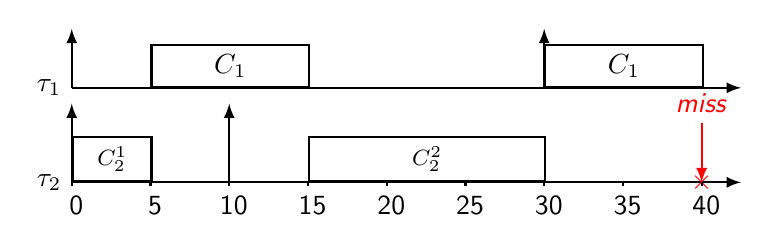
\begin{tikzpicture}[y=\uy, font=\sffamily,thick]
     
       
       
        \begin{scope}[shift={(0,0)}]
       \draw[->] (0,0)node[anchor=east,align=center] {$\tau_2$} -- coordinate (xaxis) (8.5,0);
      	\foreach \x in {3}{
      
	 	\node[task7, minimum width=6*\uy,
			anchor=south west] at ( \x, 0){\footnotesize $C_2^2$};
	}
	\foreach \x in {0}{

      		 \node[task7, minimum width=2*\uy,
anchor=south west] at ( \x, 0){\footnotesize $C_2^1$};
	 	
	}
	
	\foreach \x in {0}{
		\draw[->](\x,0) -- (\x,2)
	 		node[above] {};
	}
	\foreach \x in {2}{
		\draw[->](\x,0) -- (\x,2)
	 		node[above] {};
	}
	
	\foreach \x in {8}{
		\draw[->,red](\x,1.5) node[anchor=south] {\textit{miss}}  -- (\x,0)
			node[] {$\times$};
	 		
	}
	\foreach \x in {0,1,...,8}{
		\draw[-,below](\x,0) -- (\x,-0.1)
node[] {\pgfmathtruncatemacro\yi{5*\x} \yi};

			
	 		
	}
       \end{scope}
    
      \begin{scope}[shift={(0,2.4)}]
   
      	\draw[->](0,0) -- (0,1.5);
%\draw[->](2,0) -- (2,1);
\draw[->](6,0) -- (6,1.5);

	\foreach \x in {1,6}{
       		\node[task7, minimum width=4*\uy,
			anchor=south west] at ( \x, 0){$C_1$};
	 	
	}
	\draw[->] (0,0)node[anchor=east] {$\tau_1$} -- coordinate (xaxis) (8.5,0);


	
	
       \end{scope}
 %\draw[dotted] (10,0) -- (10,3.5);
    %  \draw[dotted] (15,0) -- (15,3.5);
     % \draw [<->] (10,3.5) -- (15,3.5)
     % 	node[anchor=south,pos=0.5] {$carry$-$in$};


      \end{tikzpicture}
\end{center}
\caption{A schedule to release the two tasks in Section~\ref{sec:wrong-periodic} simultaneously at time $0$.}
\label{fig:counterexample-FP-segment-level}
\end{figure}

{\bf Consequences:} The priority assignment algorithms in \cite{RTSS-KimANR13} and \cite{DBLP:journals/ieicet/DingTT09} use the above unsafe schedulability test to verify the priority assignments. Therefore, their results are flawed due to the unsafe schedulability test.

{\bf Solutions:} This requires to a revisit of the schedulability test of a given segmented fixed-priority priority assignment. This can be observed as a reduction to 
the generalized multiframe (GMF) task model introduced by Baruah et al.~\cite{baruah1999generalized}. A GMF task $G_i$ consisting of $m_i$ frames is characterized by the $3$-tuple $(\vec{C_i},\vec{D_i},\vec{T_i})$, where $\vec{C_i}$,$\vec{D_i}$, and $\vec{T_i}$ are $m_i$-ary vectors $(C_{i}^0,C_{i}^1,...,C_{i}^{m_i-1})$ of execution requirements, $(D_{i}^0,D_{i}^1,...,D_{i}^{m_i-1})$ of relative deadlines, $(T_{i}^0,T_{i}^1,...,T_{i}^{m_i-1})$ of minimum inter-arrival times, respectively.
In fact, from the analysis perspective, a self-suspension task $\tau_i$ under the offset enforcement is equivalent to a GMF task $G_i$,  by considering the computation segments as the frames with different separation times \cite{WC16-suspend-DATE,DBLP:journals/ieicet/DingTT09}.

However, most of the existing fixed-priority scheduling results for the GMF task model assume a unique priority level \emph{per task}. To the best of our knowledge, the only results that can be applied for a unique level \emph{per computation segment} are the utilization-based analysis in \cite{DBLP:journals/corr/ChenHL15b,huang2015mode}. 

% \subsection{Incorrect Scheduling with Slack Enforcement}
% \label{sec:wrong-slack}



%%% Local Variables:
%%% mode: latex
%%% TeX-master: "JRTS/JRTS.tex"
%%% End:

\section{Self-Suspending Tasks in Multiprocessor Synchronizations}
\label{sec:syn}

In this section, we consider the analysis of self-suspensions that arise on multiprocessors under \emph{partitioned fixed-priority (P-FP)} scheduling when tasks synchronize access to shared resources (\eg, shared I/O devices, communication buffers, or scheduler locks) with suspension-based locks (\eg, binary semaphores). Unfortunately, some of the misconceptions surrounding the analysis of self-suspensions on uniprocessors also spread to the analysis of partitioned multiprocessor real-time locking protocols. In particular, as we show with a counterexample, the analysis framework to account for the additional interference due to \emph{remote blocking} first introduced by \cite{lakshmanan-2009}, and reused in several other works~\cite{zeng-2011,bbb-2013,yang-2013,kim-2014,han-2014,carminati-2014,yang-2014},  is flawed. Finally, a straightforward solution for these problems is discussed. 

\subsection{Existing Analysis Strategies}
\label{sec:papers}

P-FP scheduling is a widespread choice in practice due to the wide support in industrial standards such as AUTOSAR, and in many RTOSs like VxWorks, RTEMS, ThreadX, \etc Under P-FP scheduling, each task has a fixed base priority and is statically assigned to a specific processor, and each processor is scheduled independently as a uniprocessor. 

Under partitioned scheduling, a resource accessed by tasks from different processors is called a \emph{global resource}, otherwise it is called a \emph{local resource}. When a job requests a global resource, it may incur \emph{remote blocking} if the global resource is held by a job on another processor. Also, a job may incur \emph{local blocking} if it is prevented from being scheduled by a resource-holding job of a lower-priority task on its local processor. 

Under suspension-based protocols, such as the \emph{multiprocessor priority ceiling protocol (MPCP)}~\cite{rajkumar-1990}, tasks that are denied to access shared resources are suspended. From the perspective of the local schedule on each processor, remote blocking, caused by external events (\ie, resource contention due to tasks on the other processors), pushes the execution of higher-priority tasks to a later time point regardless of the schedule on the local processor (\ie, even if the local processor is idle), and thus may cause additional interference on lower-priority tasks. As a result, remote blocking must be considered as a self-suspension in the analysis. In contrast, local blocking takes place only if a local lower-priority task holds the resource (\ie, if the local processor is busy). Consequently, like in the uniprocessor case, local blocking is accounted for as regular blocking, and not as self-suspension.

A safe yet pessimistic strategy, called \emph{suspension-oblivious analysis}, is to model remote blocking as computation. By overestimating the processor demand of self-suspending, higher-priority tasks, the additional delay due to deferred execution is \emph{implicitly} accounted for as part of regular interference analysis. Block et al.~\cite{block-2007} first used this strategy in the context of partitioned and global \emph{earliest deadline first (EDF)} scheduling; Lakshmanan et al.~\cite{lakshmanan-2009} also adopted this approach in their analysis of ``virtual spinning,'' where tasks suspend when blocked on a lock, but at most one task per processor may compete for a global lock at any time. However, while suspension-oblivious analysis is conceptually straightforward, it can also pessimistically overestimate response times by a factor linear in both the number of tasks and the ratio of the largest and the shortest periods~\cite{wieder-2013}.

A less pessimistic alternative to suspension-oblivious analysis is to \emph{explicitly} bound the effects of deferred execution due to remote blocking. Following this approach, Lakshmanan et al.~\cite{lakshmanan-2009} proposed the following response-time analysis framework that takes into account the amount of remote blocking to bound the worst case interference.

In Eq. \eqref{eqn:wcrt} below, let $B_k^r$ denote an upper bound on the maximum remote blocking that a job of $\tau_k$ incurs, let $C_k^{\ast} = C_k + B_k^r$, and let $\fun{hp(k)}$ and $\fun{lp(k)}$ denote the tasks with higher and lower priority than $\tau_k$, respectively. Furthermore, let $P(\tau_k)$ denote the tasks that are assigned on the same processor as $\tau_k$, and $s_k$ is the maximum number of critical sections of $\tau_k$, and $C_{l,j}^{\prime}$ is an upper bound on the execution time of the $j$\xth critical section of $\tau_l$. It was claimed in \cite{lakshmanan-2009} that, if $R_k^{n+1} = R_k^n \leq D_k$ for some $n > 0$, where $R_k^0 = C_k^{\ast}$ and
\begin{equation}
\label{eqn:wcrt}
R_k^{n+1} = C_k^{\ast} + \sum_{\tau_i \in \fun{hp(k)} \cap P(\tau_k)} \left \lceil \frac{R_k^n + B_i^r}{T_i} \right \rceil \cdot C_i + s_k \sum_{\tau_l \in \fun{lp(k)} \cap P(\tau_k)} \max_{1 \leq j < s_l} C_{l,j}^{\prime}
\end{equation}
then task $\tau_k$ is schedulable and its response time is bounded by $R_k^n$. This  response-time analysis framework~\cite{lakshmanan-2009} was subsequently reused in
\begin{itemize}
\item \cite{zeng-2011} (Equation 9), \cite{han-2014}(Equation 5), and \cite{yang-2014} (Section 2.5) for the MPCP analysis, and
\item \cite{yang-2013} (Equation 6), \cite{bbb-2013} (Equation 1), \cite{carminati-2014} (Equations 3, 12, and 16), and \cite{kim-2014} (Equation 6) to guide the analysis for certain other suspension-based locking protocols.
\end{itemize}

In Eq. \eqref{eqn:wcrt}, the additional interference on $\tau_k$ due to the lock-induced deferred execution of higher-priority tasks is captured by the term ``$+ B^r_i$'' in the interference bound  $\left \lceil \frac{R_k^n + B_i^r}{T_i} \right \rceil \cdot C_i$. This is very similar to the misconception of self-suspending task systems presented in Section~\ref{sec:wrong-jitter-dynamic} by treating the remote blocking as self-suspension. For completeness, we explain why this fails to guarantee a safe response-time bound in certain corner cases by giving a counterexample in the following subsection.

\subsection{A Counterexample}
\label{sec:counterexample}

We show the existence of a schedule in which a task that is considered schedulable according to the analysis in \cite{lakshmanan-2009} is in fact unschedulable.

%\begin{figure}[!ht]
\begin{center}
\includegraphics[width=12cm]{Counterexample}
\caption{An example schedule in which $\tau_3$ misses a deadline. 
}
\label{fig:counterexample_protocol}
\end{center}
\end{figure}


\begin{table}
\centering
    \begin{tabular}{|c|c|c|c|c|c|} 
 \hline
        $\tau_k$ & $C_k$ & $T_k$ ($= D_k$) & $s_k$ & $C_{k,1}^{\prime}$ & Processor\\
        \hline
        $\tau_1$ & 2             & 6  & 0 & $-$ & $1$\\ 
        $\tau_2$ & $4+6\epsilon$ & 13 & 1 & $5\epsilon$& $5$\\
        $\tau_3$ & $\epsilon$    & 14 & 0 & $-$ & $1$\\
        $\tau_4$ & 7             & 14 & 1 & $4-4\epsilon$ & $2$\\ 
        \hline
    \end{tabular}
    \caption{Task parameters for the counter example in Section~\ref{sec:counterexample}.}
    \label{table:parameters}
\end{table}

Consider four implicit deadline sporadic tasks ${\tau_1, \tau_2, \tau_3, \tau_4}$ (with parameters listed in Table \ref{table:parameters}), ordered by a decreasing order of priority, that are scheduled on two processors using P-FP scheduling. Tasks $\tau_1$, $\tau_2$ and $\tau_3$ are assigned to processor 1, while task $\tau_4$ is assigned to processor 2. Each job of $\tau_2$ has a critical section guarded by a global shared resource $\res_1$  ($s_2 = 1$), in which the length of the critical section is at most $5\varepsilon$, $0 < \varepsilon \leq 1/3$, i.e., $C_{2,1}^{\prime} = 5\varepsilon$. 
Each job of $\tau_4$ has a critical section guarded by a global shared resource $\res_1$  ($s_4 = 1$), in which the length of the critical section is at most $4-4\varepsilon$, i.e., $C_{4,1}^{\prime} = 4-4\varepsilon$. 

Consider the response-time of $\tau_3$. Since $\tau_3$ does not access any global resource and it is the lowest-priority task on processor $1$, it does not incur any global or local blocking (\ie, $B_3^r = 0$ and $s_3 \sum_{\tau_l \in \fun{lp}(3) \cap P(\tau_3)} \max_{1 \leq j < s_l} C_{l,j}^{\prime} = 0$). With regard to the remote blocking incurred by each higher-priority task, we have $B_1^r = 0$ because $\tau_1$ does not request any global resource. Further, each time when a job of $T_2$ requests $\res_1$, it may be delayed by $\tau_4$ for a duration of at most $4-4\varepsilon$. Thus the maximum remote blocking of $\tau_2$ is bounded by $B_2^r = C_{4,1}^{\prime} = 4-4\varepsilon$.\footnote{In general, the upper bound on blocking of course depends on the specific locking protocol in use, but in this example, by construction, the stated bound holds under any reasonable locking protocol. Recent surveys of multiprocessor semaphore protocols may be found in \cite{bbb-2013,yang-2015}.} Therefore, according to Eq. \eqref{eqn:wcrt}, we have
\begin{align*}
& R_3^0 = \varepsilon + 0 = \varepsilon, \\
& R_3^1 = \varepsilon + \left \lceil \frac{\varepsilon + 0}{6} \right \rceil \cdot 2 + \left \lceil \frac{\varepsilon + 4 - 4\varepsilon}{13} \right \rceil \cdot (4+6\varepsilon) =  6+7\varepsilon, \\
& R_3^2 = \varepsilon + \left \lceil \frac{6+7\varepsilon + 0}{6} \right \rceil \cdot 2 + \left \lceil \frac{6+7\varepsilon + 4-4\varepsilon}{13} \right \rceil \cdot (4+6\varepsilon) = 8+7\varepsilon, \\
& R_3^3 = \varepsilon + \left \lceil \frac{8+7\varepsilon + 0}{6} \right \rceil \cdot 2 + \left \lceil \frac{8+7\varepsilon + 4-4\varepsilon}{13} \right \rceil \cdot (4+6\varepsilon) = 8+7\varepsilon.
\end{align*}


\begin{figure}[t]
\centering
\def\uxfpga{0.4cm}
\scalebox{0.9}{
\begin{tikzpicture}[x=\uxfpga,y=\uy,auto, thick]
	\draw[->] (-0.4,0) -- coordinate (xaxis) (24,0) node[anchor=north]{$t$};
    \foreach \x in {0,2,...,22}{
         \draw[-,below](\x,0) -- (\x,-0.3) node[] {\pgfmathtruncatemacro\yi{\x} \yi};
    }
    	\foreach \x in {0,1,...,21}{
         \draw[-,very thin,lightgray, dashed](\x,0.3) -- (\x,9.75);
	}	
	\foreach \x in {-0.4,22}{
		\draw[-,thin,gray] (\x,0) -- (\x,2.25);
		\draw[-,thin,gray] (\x,2.7) -- (\x,9.75);
	}
	\foreach \y in {2.25,2.7,9.75}{
		\draw[-,thin,gray] (-0.4,\y) -- (22,\y);
	}
	\foreach \y in {3,5,7}{
		\draw[] (0,\y) -- (22,\y);
	}	
    \node[anchor=east] at (13, 1.5) {Processor 1};
    \node[anchor=east] at (13, 9.25) {Processor 2};

	\begin{scope}[shift={(0,0)}]
	    \node[anchor=east] at (-0.5, 0.5) {$\tau_4$};
		\foreach \x in {1,15}{
			\draw[->] (\x,0) -- (\x,1.75);
        		\node[task7, minimum width=\uxfpga, anchor=south west] at (\x, 0){\footnotesize};         
        		\node[task9, minimum width=3.4*\uxfpga, anchor=south west] at (\x+1, 0){\footnotesize};
        		\draw[] (\x+4.4,1.03)--(\x+6,1.03);
        		\draw[] (\x+6,0)--(\x+6,1.03);
		}
	\end{scope}
        
    \begin{scope}[shift={(0,3)}]
		\node[anchor=east] at (-0.5, 0.5) {$\tau_3$};    
    		\draw[->] (6,0) -- (6,1.75);
    		\draw[<-,red] (20,0) -- (20,1.2);
    		\node[anchor=east,red] at (21, 1.5) {miss};
    	\end{scope}
        
    \begin{scope}[shift={(0,5)}]    
        \node[anchor=east] at (-0.5, 0.5) {$\tau_2$};
        \draw[->] (0,0) -- (0,1.75);
        \draw[->] (13,0) -- (13,1.75);
        \foreach \y in {0.3,0.5,0.7}{
        		\draw[] (2.15,\y) -- (5.5,\y);
        	}
        \draw[] (2,1.03)--(2.15,1.03);
        \draw[] (2.15,0)--(2.15,1.03);
        \draw[] (2,0) -- (2,1.03);
        \node[task9, minimum width=0.1*\uxfpga, anchor=south east] at (6.05, 0){\footnotesize};
        \node[task7, minimum width=4*\uxfpga, anchor=south west] at (8, 0){\footnotesize}; 
        \draw[] (14,1.03)--(14.15,1.03);
        \draw[] (14,0)--(14,1.03);
        \node[task9, minimum width=0.1*\uxfpga, anchor=south west] at (14.15, 0){\footnotesize};
        \draw[] (14.7,1.03)--(18,1.03);
        \draw[] (18,0)--(18,1.03);
        \node[task7, minimum width=0.1*\uxfpga, anchor=south west] at (20, 0){\footnotesize};
	\end{scope}
	
	\begin{scope}[shift={(0,7)}]
        \node[anchor=east] at (-0.5, 0.5) {$\tau_1$}; 
        \foreach \x in {0,6,...,18}{
        		\draw[->] (\x,0) -- (\x,1.75);
		    \node[task7, minimum width=2*\uxfpga, anchor=south west] at (\x, 0){\footnotesize};
		}
	\end{scope}
\end{tikzpicture}}       
\caption{A schedule where $\tau_3$ misses a deadline.}
\label{fig:counterexample_protocol}
\end{figure}

\ifpaper
%\begin{figure}[t]
%  \centering
%  \includegraphics[width=0.85\linewidth]{../figures/Counterexample1/Counterexample1.pdf}
%  \caption{An example schedule where $\tau_3$ misses a deadline.}\label{fig:counterexample_protocol}
%\end{figure}
 \fi

As a result, $R_3 = 8+7\varepsilon < 14 = D_3$, and $\tau_3$ is considered to be schedulable according to the analysis in \cite{lakshmanan-2009}. However, there exists a schedule, shown in Fig. \ref{fig:counterexample_protocol}, which is perfectly legal, where a job of task $\tau_3$  is released at time $6$ and misses its absolute deadline at time $20$. This implies that Eq. \eqref{eqn:wcrt} does not always yield a sound response-time bound. 

The misconception here is to use the remote blocking of each higher-priority task (\ie, $B_i^r$) in a similar way as release jitter. However, it is not sufficient to count the duration of remote blocking as release jitter, as already explained in Section~\ref{sec:wrong-jitter-dynamic}.

\subsection{Incorrect Time Request Analysis With Global Resource Sharing}

A related problem affects an \emph{interface-based analysis}  proposed by \cite{NBN:11}. Targeting \emph{open} real-time systems with globally shared resources (\ie, systems where the final task set composition is not known at analysis time, but tasks may share global resources nonetheless), the goal of the interface-based analysis is to extract a concise abstraction of the constraints that need to be maintained in order  to guarantee the schedulability of all tasks. In particular, the analysis seeks to determine the \emph{maximum tolerable blocking time}, denoted $\fun{mtbt}_k$, that a task $\tau_k$ can tolerate without missing its deadline. 

Recall from classic uniprocessor time-demand analysis \cite{lehoczky-1989} that, \emph{in the absence of jitter or self-suspensions}, a task $\tau_k$ is considered schedulable if
\begin{equation}
\label{eqn:rbf-1}
\exists t \in (0,D_k]: \fun{rbf_{FP}}(k,t) \leq t, 
\end{equation}
where $\fun{rbf_{FP}}(k,t)$ is the \emph{request bound function} of $\tau_k$, which is given by

\begin{equation}
\label{eqn:rbf-2}
\fun{rbf_{FP}} = C_k + B_k + \sum_{\tau_i \in \fun{hp}(k)} \left \lceil \frac{t}{T_i} \right \rceil \cdot C_i.
\end{equation}

Starting from Eq. \eqref{eqn:rbf-1}, Nemati et al.~\cite{NBN:11} first  replaced $\fun{rbf_{FP}}(k,t)$ with its definition, and then substituted  $B_k$ with $\fun{mtbt}_k$. Solving for $\fun{mtbt}_k$ yields:
\begin{equation}
\label{eqn:bloc-tolerate}
\fun{mtbt}_k = \max_{0<t \leq D_k} \left( t - ( C_k + \sum_{\tau_i \in \fun{hp}(k)} \left \lceil \frac{t}{T_i} \right \rceil \cdot C_i ) \right).
\end{equation}

However, based on the example in Section \ref{sec:counterexample}, we can immediately infer that Eq. \eqref{eqn:rbf-1} and Eq. \eqref{eqn:rbf-2}, which ignore the effects of deferred execution due to remote blocking, are unsound in the presence of global locks. Consider $\tau_3$ in the previous example (with parameters listed in Table \ref{table:parameters}). According to Eq. \eqref{eqn:bloc-tolerate}, we have $\fun{mtbt}_3 \geq 12 - (\epsilon + \lceil 12 / 6 \rceil \cdot 2 + \lceil 12 / 13 \rceil \cdot (4+6\epsilon)) = 4-7\epsilon$ (for $t=12$), which implies that $\tau_3$ can tolerate a maximum blocking time of at least $4-7\epsilon$ without missing its deadline. However, this is not true since $\tau_3$ can miss its deadline even without incurring any blocking, as shown in Fig. \ref{fig:counterexample_protocol}. 

\subsection{A Safe Response Time Bound}
\label{sec:safe_bound}

In Eq. \eqref{eqn:wcrt}, the remote blocking of each higher-priority task (\ie, $B_i^r$) is counted in a similar way as release jitter. However, it is not sufficient to count the duration of remote blocking as release jitter, as already explained in Section~\ref{sec:wrong-jitter-dynamic}. A straightforward fix is thus to replace $B_i^r$, in the ceiling function (\ie, the second term in Eq. \eqref{eqn:wcrt}), with a larger value such as $D_i$ (as discussed in Section~\ref{sec:wrong-jitter-dynamic}) or $R_i - C_i$ if $R_i \leq T_i$. Similarly, replacing $\sum_{\tau_i \in \fun{hp}(k)} \lceil t / T_i \rceil \cdot C_i$ in Eq. \eqref{eqn:rbf-2} and Eq. \eqref{eqn:bloc-tolerate} with $\sum_{\tau_i \in \fun{hp}(k)} \lceil (t+D_i) / T_i \rceil \cdot C_i$ or $\sum_{\tau_i \in \fun{hp}(k)} \lceil (t+R_i-C_i) / T_i \rceil \cdot C_i$ can fix the corresponding over-optimistic problem.

Further, since \cite{zeng-2011,bbb-2013,yang-2013,kim-2014,han-2014,carminati-2014,yang-2014} reviewed in Section \ref{sec:papers} merely reused the over-optimistic analysis approach introduced in \cite{lakshmanan-2009} (\ie, reusing $\left \lceil \frac{R_k^n + B_i^r}{T_i} \right \rceil \cdot C_i$ as an interference bound of $\tau_i$ on $\tau_k$), the stated fix as potential solutions may be used to correct the response-time tests in these papers without additional changes.


  
  


%%% Local Variables:
%%% mode: latex
%%% TeX-master: "JRTS/JRTS.tex"
%%% End:


  
\section{Soft Real-Time Self-Suspending Task Systems}
\label{sec:soft-realtime}

For a hard real-time task, its deadline must be met; while for a soft real-time task, missing some deadlines can be tolerated. We assume a well-studied soft real-time notion, in which \emph{a soft real-time task is schedulable if its tardiness can be provably bounded}. (Such bounds would be expected to be reasonably small.) A task's tardiness is defined to be its maximum job tardiness, which is calculated as $0$ if the job finishes before its absolute deadline and a job's completion time minus the job's absolute deadline otherwise.
The schedulability analysis techniques on soft real-time self-suspending task systems can be categorized into two categories: suspension-oblivious analysis v.s. suspension-aware analysis.

\subsection{Suspension-Oblivious Analysis}
\label{sec:sus-oblivious-soft}

 The suspension-oblivious analysis simply treats the suspensions as computation, as also explained in Section~\ref{sec:oblivious}. From \cite{Devi2005,Leontyev072}, tardiness is bounded under a pure computational task system (no suspensions) provided $\sum_{i=1}^{n} (C_i+S_i)/T_i \leq M$, where $M$ is the number of processors in the system. A downside of treating all suspensions as computation is that this causes utilization bound to be $\sum_{i=1}^{n} S_i/T_i$ higher, which in many cases may cause total utilization to exceed $M$.  This suspension-oblivious approach causes an $O(n)$ utilization loss, where $n$ denotes the number of self-suspending tasks in the system. 
 Due to the $O(n)$ utilization loss, the suspension-oblivious analysis is pessimistic. 

\subsection{Suspension-Aware Analysis}
\label{sec:sus-aware-soft}

Several recent works have been conducted to reduce this utilization loss by focusing on deriving suspension-aware analysis. The main difference between the suspension-aware and the suspension-oblivious analysis is that, under the suspension-aware analysis, suspensions are specifically considered in the task model as well as in the schedulability analysis. These works on conducting suspension-aware analysis techniques for soft real-time suspending task systems on multiprocessors are mainly done by Liu and Anderson~\cite{Liu3,Liu4,Liu5,Liu9,Liu11}. The main idea behind these techniques is that treating all suspensions as computation is pessimistic, instead, smartly treating a selective minimum set of suspensions as computation can significantly reduce the pessimism in the schedulability analysis. This is also the main reason why these techniques can significantly improve the suspension-oblivious approach in most cases.

In 2009, Liu and Anderson derived the first such schedulability test~\cite{Liu3}, where they showed that in preemptive sporadic systems, bounded tardiness can be ensured by developing suspension-aware analysis under global EDF scheduling and global first-in-first-out (FIFO) scheduling. Specifically it is shown in \cite{Liu3} that tardiness in such a system is bounded provided 
\begin{equation}\label{eq:constraint} U_{sum}^s + U_L^c < (1-\xi_{max}) \cdot M , \end{equation}
where $U_{sum}^s$ is the total utilization of all self-suspending tasks, $c$ is the number of computational tasks (which do not self-suspend), $M$ is the number of processors, $U_L^c$ is the sum of the $\min(M-1,c)$ largest computational task utilizations, and $\xi_{max}$ is a parameter ranging over $[0,1]$ called the \textit{maximum suspension ratio}, which is defined to be the maximum value among all tasks' suspension ratios. For any task $\tau_i$, its suspension ratio, denoted $\xi_i$, is defined to be $\xi_i = \dfrac{S_i}{S_i+C_i}$, where $S_i$ is the suspension length of task $\tau_i$ and $C_i$ is its execution cost.  Significant utilization loss may occur when using (\ref{eq:constraint}) if $\xi_{max}$ is large. Unfortunately, it is unavoidable that many self-suspending task systems will have large $\xi_{max}$ values. For example, consider an implicit-deadline soft real-time task system with three tasks scheduled on two processors: $\tau_1$ has $C_1=5, S_1=5$, and a $T_1=10$, $\tau_2$ has $C_2=2, S_2=0$, and $T_2=8$, and $\tau_3$ has $C_3=2, S_3=2$, and $T_3=8$. For this system, $U_{sum}^s = U_1+U_3= \dfrac{5}{10} + \dfrac{2}{8} = 0.75$, $U_L^c = U_2 = \dfrac{2}{8} = 0.25$, $\xi_{max} = \xi_1 = \dfrac{5}{5+5} = 0.5$. Although the total utilization of this task system is only half of the overall processor capacity, it is not schedulable using the prior analysis since it violates the utilization constraint in (\ref{eq:constraint}) (since $U_{sum}^s+U_L^c =1=(1-\xi_{max}) \cdot M$).

In a follow-up work \cite{Liu5}, by observing that the utilization loss seen in (\ref{eq:constraint}) is mainly caused by a large value of $\xi_{max}$, Liu and Anderson presented a technique that can effectively decrease the value of this parameter, thus increasing schedulability. 
% They show that this can be done by treating \textit{partial} suspensions as computation. That is, they consider intermediate choices between the two currently-available extremes of treating \textit{all} (as is commonly done) or \textit{no} (using the analysis in ???Liu093) suspensions as computation. 
This approach is often able to decrease $\xi_{max}$ at the cost of at most a slight increase in the left side of (\ref{eq:constraint}). 
% The authors present both a linear programming solution for determining how much suspension time to be treated as computation as well as an optimal algorithm that runs in $O((N^s)^2)$ time, where $N^s$ is the number of self-suspending tasks. The authors analyze the schedulability improvement brought by the proposed approach via an experimental study involving randomly-generated task systems. In all scenarios considered in this study, this approach was able to improve schedulability, and in most scenarios, by a substantial margin. 
In \cite{Liu4}, Liu and Anderson  showed that any task system with self-suspensions, pipelines, and
non-preemptive sections can be transformed for analysis purposes into a system with only self-suspensions \cite{Liu4}. The transformation process treats delays caused by pipeline-based precedence constraints and non-preemptivity as self-suspension delays.
In \cite{Liu9,Liu11}, Liu and Anderson derived the first soft real-time schedulability test for suspending task systems that analytically dominates the suspension-oblivious approach.
 % Specifically, they show that an $O(M)$ utilization loss (where $M$ is the number of processors) can be achieved under a new suspension-aware analysis technique. 



%%% Local Variables:
%%% mode: latex
%%% TeX-master: "JRTS/JRTS.tex"
%%% End:


  
\section{Hardness Review of Self-Suspending Task Models}
   EDF/RM not optimal \cite{Ridouard_2004} 
   
\begin{itemize}
\item \textbf{The complexity class of scheduling policies}
\item \textbf{Open problems for schedulability analysis, etc.}
\end{itemize}
  
\section{Rule of Thumb for Handling Self-Suspending Task Systems}
\section{Short Summary of the Errors and Mistakes in the State of the Art}
  
  A table to list the erratum that can be found and the reasons for the mistakes and errors.

\newpage

\chapter*{Changelog}

In addition to some rewordings, the following significant changes have
been made after the first version:
\begin{enumerate}
\item Eq.~\eqref{eq:dynamic-flawed} is revised with
  $\ceiling{\frac{R_k + S_{\textcolor{blue}{i}}}{T_i}}$  since the first
  version used $\ceiling{\frac{R_k + S_{\textcolor{red}{k}}}{T_i}}$
  with a typo.
\item Eq.~\eqref{eqn:wcrt} is revised with \textcolor{blue}{$s_k+1$} instead of
  \textcolor{red}{$s_k$} since the notation used in this report is different
  from the original source in \cite{lakshmanan-2009}.
\item The misconception in Section~\ref{sec:wrong-periodic} is 
  listed as a solved issue due to the errata \cite{Kim2016}, published
  in August 2016.
\item Section~\ref{sec:model-interfering-unified} is added due to a
  recent result in \cite{ChenECRTS2016-suspension}, published in July 2016
\item Section~\ref{sec:wrong-jitter-convert-sporadic} is added due to
  a recent errata \cite{nelissen-errata-ECRTS15}, published in
  February 2017.
\item Chapter~\ref{sec:hardness} is updated due to the latest result
  in \cite{RTSS2016-suspension,DBLP:conf/rtns/MohaqeqiE016}.
\item Papers published in 2016 are added and discussed.
\end{enumerate}
(All the indexes are based on the latest version, i.e., 2nd ver.)


\bibliographystyle{abbrv}
\bibliography{../bibliography/biblio}{}


%\setlength\bibitemsep{1pt}
%\printbibliography[maxnames=999]
%\printbibliography
%
\end{document}
% ********************************************************************
